\chapter{Corrections}
\label{chap:corr}

\section{Trigger efficiency}
Trigger efficiency of $\pprefMBtrig$ for the $\pprefSample$ could not be determined data-driven, due to the control trigger missing on the menu and resurrection option being turned off. For the $\OO$, it will be determined using the control trigger HLT\_no\_alg\_L1\_RD0, which will be present on the menu. In Run 1, for $\pPb$ \cite{pPb_mbsptrk_trigger} the trigger efficiency $\epsilon_{\mathrm{trigger, pp}}$ for $\pprefMBtrig$ was determined to be fully efficient for events with loose track multiplicity > 2 and with $\epsilon_{\mathrm{trigger, pp}} = 99.6\pm0.3\%$ for multiplicity 2. This analysis takes these efficiencies and applies them at the closest level of quality in our selection (loosePrimary + d0).

For events with fewer tracks, there is no reference. However, events with 0 (loosePrimary + d0) tracks - making up 0.2\% of events in the studied sample - have in 99.2\% cases 0 vertices in the event, thus they do not change the $\RAA$ determination. Therefore, for events with 0 tracks, no efficiency correction is applied as it would have a negligible effect on the final spectrum.

In case of events with (loosePrimary + d0) 1 track - making up 0.7\% of events in the studied sample - there are 90 \% events with 0 vertices, and the remaining 10 \% of events have 1 vertex. Again, the overall contribution of these events to the spectrum is negligible, given the average number of vertices is 2.5 and the average number of good tracks is 66. Thus, no correction on the trigger efficiency is applied.

\section{Vertex reconstruction efficiency}
The vertex reconstruction efficiency $\epsilon_{\mathrm{vtx}}$ is determined in a data-driven approach as the ratio of triggered events with a reconstructed vertex to the total number of triggered events as a function of the number of tracks in our fiducial space using the low-$\mu$ data. The measured efficiency is plotted on Figure~\ref{fig:vrtx_eff}. Efficiency is shown for various diffraction modes based on the $\forwardgap$ cut as a function of the number of tracks in the analysis fiducial space. Inclusively, the efficiency is $\epsilon_{\mathrm{vtx}} = 95.7\%$. Since the $\RAA$ is measured using the number of vertices, this correction must be applied to every vertex. One can correct for $\epsilon_{\mathrm{vtx}}$ differentially based on $\ntrk$, when retrieving events with 1 vertex reconstructed as events with 0 vertices. However, in the case of higher $\mu$, the only option is to correct the total number of vertices in the analysis $\nvtx$. This is possible if one considers vertex reconstruction independent, and thus, its efficiency is also independent. 

\begin{figure}
    \centering
    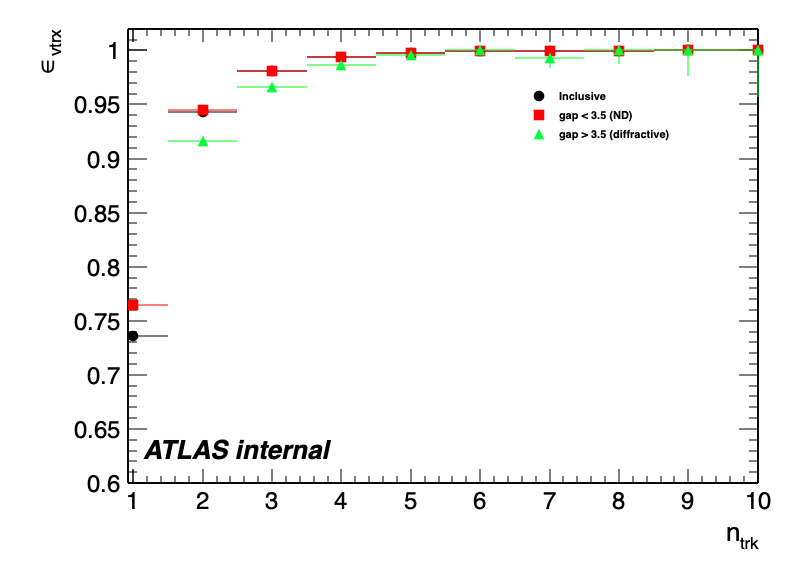
\includegraphics[width=0.5\linewidth]{images/vrtx_eff.png}
    \caption{Vertex reconstruction efficiency}
    \label{fig:vrtx_eff}
\end{figure}


%{
%\red Found events with $0$ vertices yet some number of tracks (see fig.~\ref{fig:trkpt_novtx}). There seems to be a clear threshold at 0.4, indicating that to create a vertex, there should be a track with $p_T$ more than 0.4 GeV. Figure out how many actual collisions we miss by that (e.g., if we keep those tracks)? Monte-Carlo?

%\begin{figure}
%    \centering
%    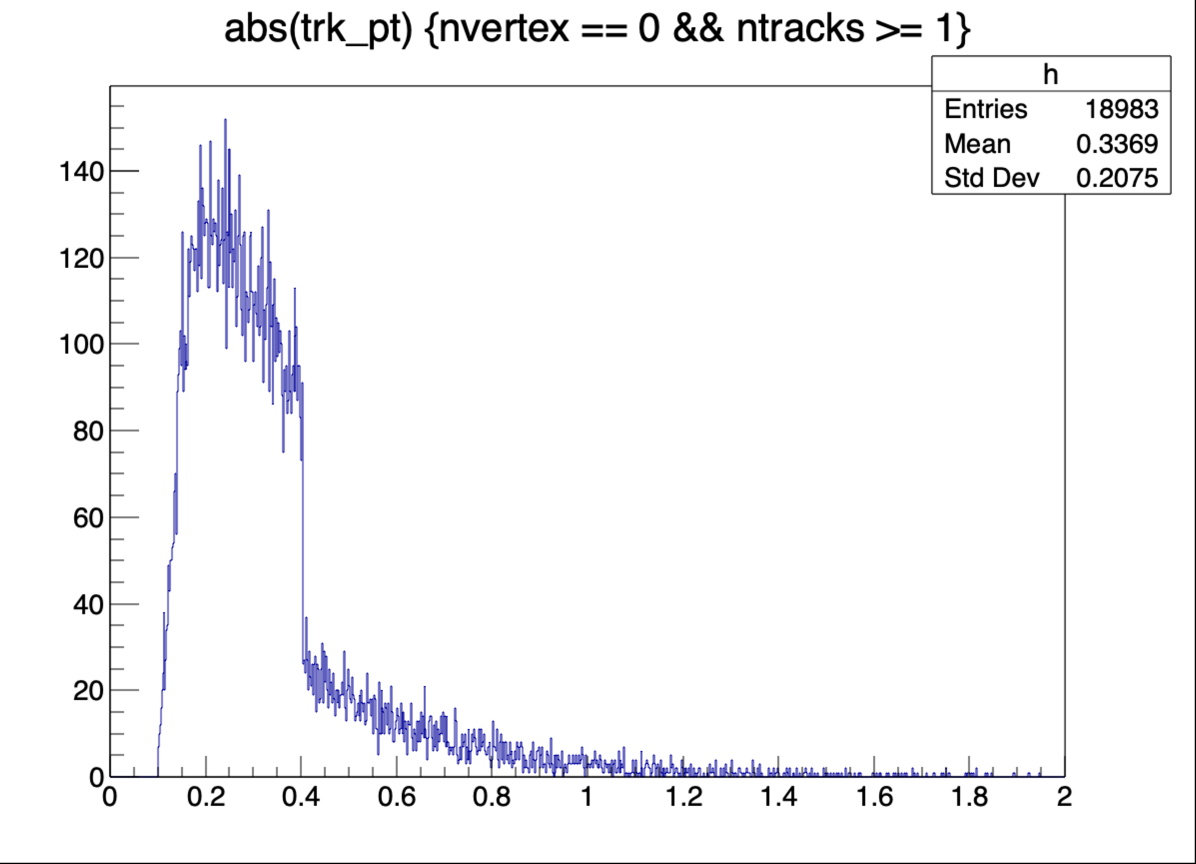
\includegraphics[width=0.5\linewidth]{images/trkpt_novtx.png}
%    \caption{Pt of tracks with events with no vertices}
%    \label{fig:trkpt_novtx}
%\end{figure}

%}

% poisson-vertex method


\section{Pileup}
\label{sec:vertex_merging}

Due to the fact that several collisions can occur during the same bunch crossing, for a number of collisions that happen close to each other, the reconstruction algorithm may fail to resolve their vertices~\cite{ATLAS:2016nnj}. This results in two effects. The number of vertices is not properly determined. The position of the merged vertex is shifted with respect to the positions of the original vertices. Although the merging happens in 3D, the main effect is in $z$ coordinates because of the much longer $z$-dimension of the beam spot. 

One can estimate the number of merged vertices directly from the data and correct for it using the following procedure. 

Distribution of $z$-distances between all pairs of vertices is shown in the left panel of Figure~\ref{fig:vtx_z_dist}. 
\begin{figure}[h]
\centering
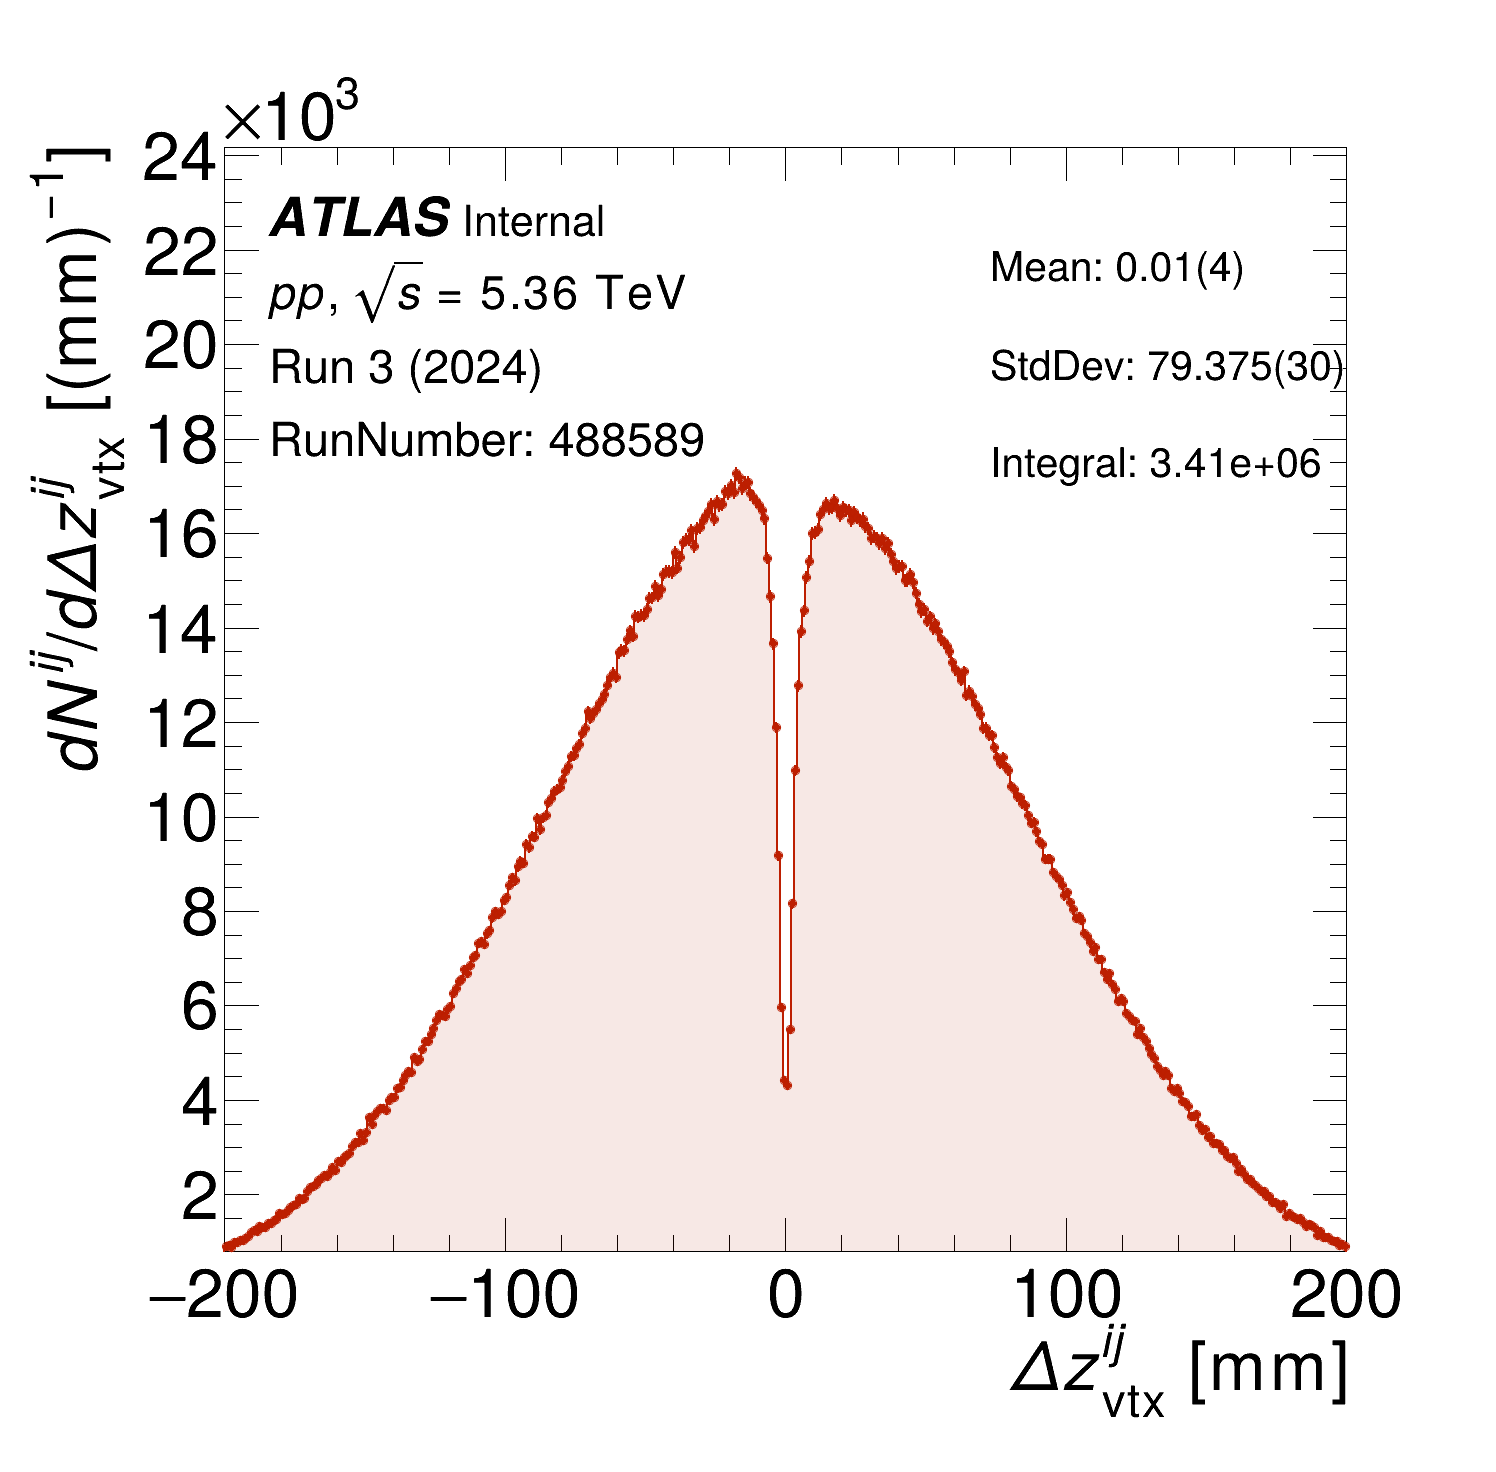
\includegraphics[width=0.26\textwidth]{images/vertex_z_dist_488589.png}
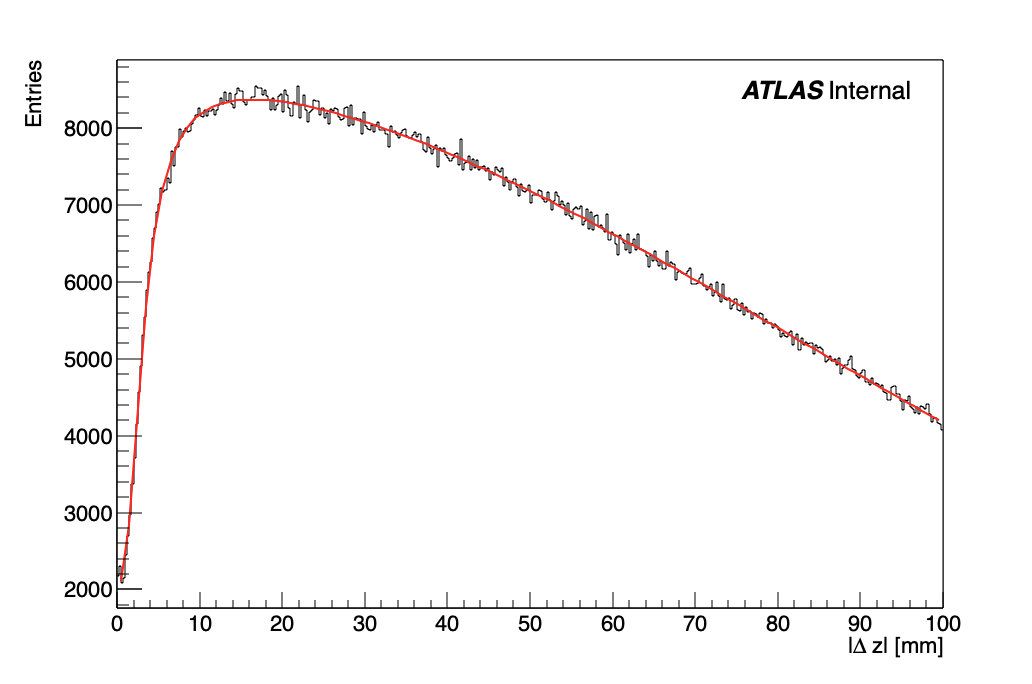
\includegraphics[width=0.38\textwidth]{images/fit_bw_z.png}
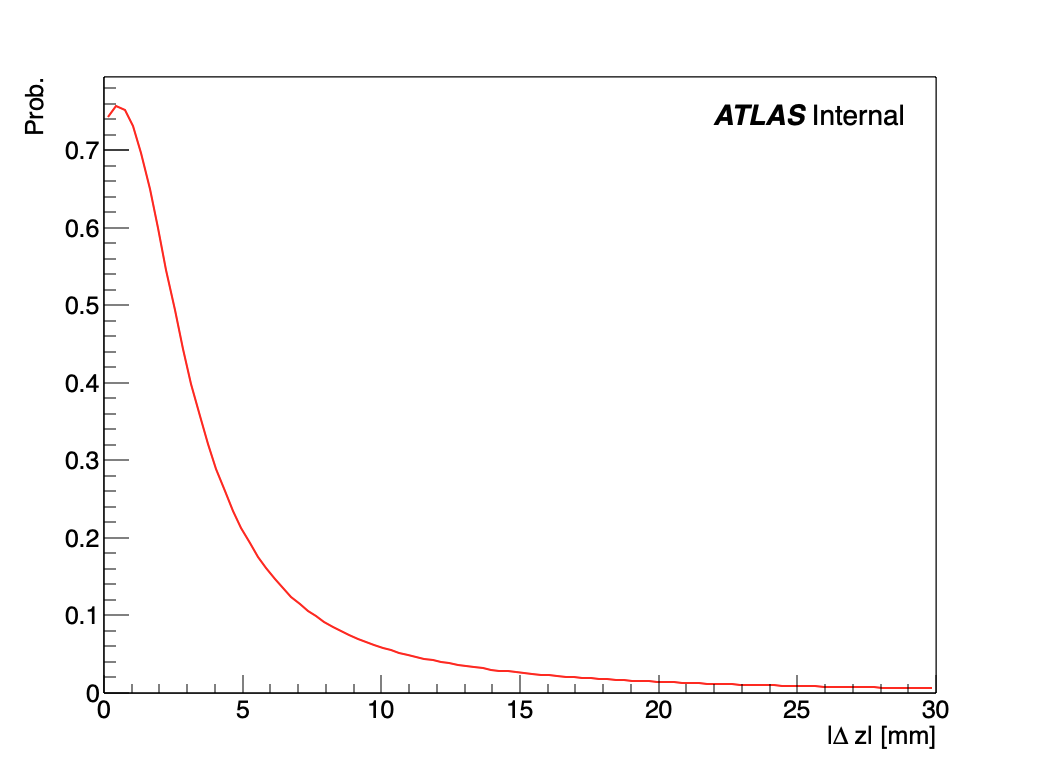
\includegraphics[width=0.34\textwidth]{images/fit_merg_prob.png}
\caption{Left: Distance $\Delta z^{ij}$ between vertices in chunk of run 488589, with $\langle \mu \rangle \sim 4.0$. Middle: Symmetrized distribution $|\Delta z_\text{vtx}^{ij}|$ and fit with $f(\Delta z)$. Right: Merging probability function $\mathcal{P}(\Delta z)$. 
%{\red suggest to improve the quality of these plots so that they look better in a line.}
%{\blue Can one improve plotting the function such that it does not change derivative at low values, but has it identically equal to zero? Knowing ATLAS, this curve is "an invited question". I'd avoid that.}
    \label{fig:vtx_z_dist}}
\end{figure}
The drop around zero demonstrates the effect of vertices merging. The slight asymmetry of the distribution might come from the internal ordering of the vertex coordinates. The distribution is symmetrized by taking the absolute value of the vertex distance as shown in the middle panel of the Figure. Symmetrized distribution is 
%the "dip" region ($|\Delta z^{ij}_\text{vtx}|< $ \qty{10}{\mm}) is shown in Figure~\ref{fig:vertex_dz_fit}.  
%  \begin{figure}[h]
%      \centering
%      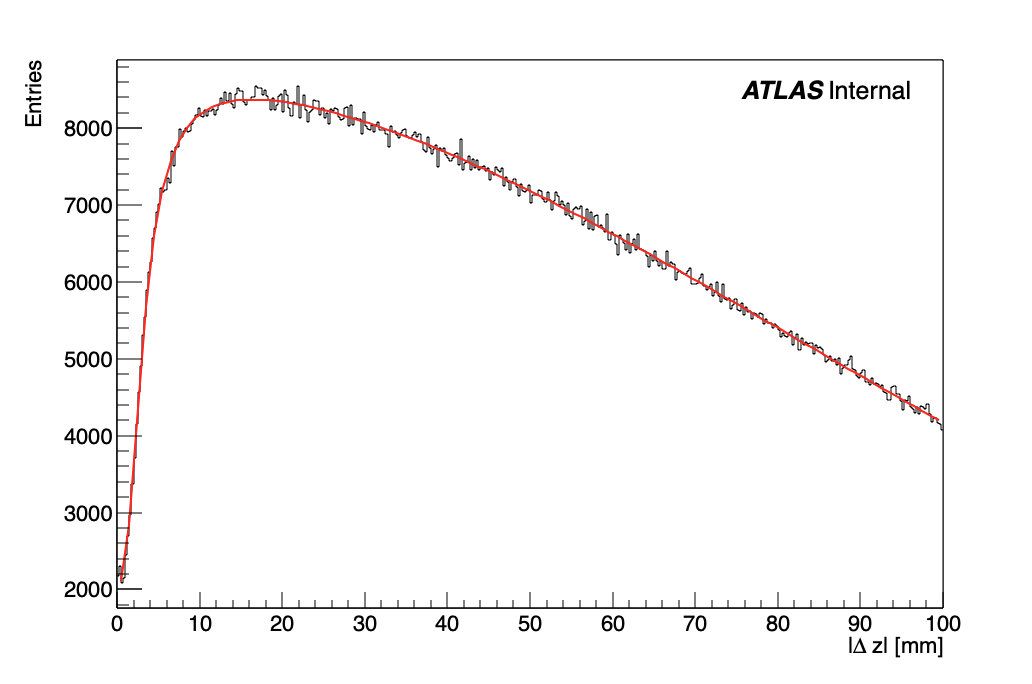
\includegraphics[width=0.45\linewidth]{images/fit_bw_z.png}
%      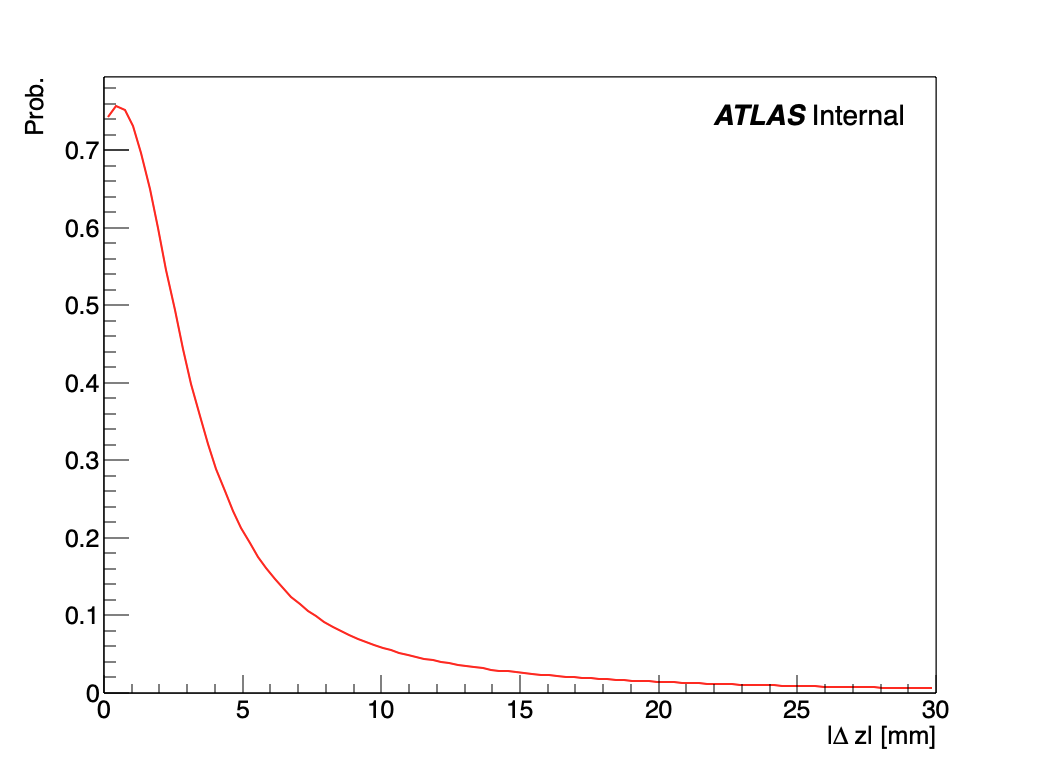
\includegraphics[width=0.45\linewidth]{images/fit_merg_prob.png}
%      \caption{Left: symmetrized distribution $|\Delta z_\text{vtx}^{ij}|$ and fit with $f(\Delta z)$. Right: Merging probability function $\mathcal{P}(\Delta z)$ }
%      \label{fig:vertex_dz_fit}
%  \end{figure}
%  is fitted to the function $f_1$ and the rest with $f_2$ (see below). After such estimation of initial parameters, the total function
  \begin{equation}
      f(\Delta z) = \frac{A_1}{2\pi}\frac{\Gamma}{(\Delta z - M)^2 + \Gamma^2/4} + A_2\exp{\left(-\frac{(\Delta z - \mu)^2} {\sigma^2} \right)} = f_1(\Delta z) + f_2(\Delta z)
  \end{equation}
  %is fitted to the distribution 
  in the range $[0,70]$ mm. Extracted fit ($\chi^2/\text{n.d.f}\approx 1$) parameters are listed in Table~\ref{tab:bw_gaus_pars} 
  % {\red is that important? I think showing the fit is perfectly enough, but if you want to keep it, I suggest commenting on its stability for different values of $\mu$. This universality is rather important for the analysis, but the fit values are not so much. They would change run-by-run if the width of the \zvtx changes.} 
  \begin{table}[h]
      \centering
      \caption{Parameters of $f(\Delta z)$}
      \begin{tabular}{c|c}
           Parameter & Value  \\
           \hline
           % NOT ROUNDED
           % $A_1$ & $-58354.6 \pm 1037.83$ \\
           % $M$ & $0.531183 \pm 0.0267741$ \\
           % $\Gamma$ & $5.53881 \pm 0.0786292$ \\
           % $A_2$ & $8838.9 \pm 36.3994$ \\
           % $\mu$ & $-4.77708 \pm 1.13528$ \\
           % $\sigma$ & $85.6301 \pm 0.833025  $ \\
           % ROUNDED
           $A_1$ & $(-584\pm 10)\times10^2$ \\
           $M$ [mm] & $0.531 \pm 0.027$ \\
           $\Gamma$ [mm] & $5.54 \pm 0.08$ \\
           $A_2$ & $8839 \pm 40$ \\
           $\mu$ [mm] & $-4.8 \pm 1.1$ \\
           $\sigma$ [mm] & $85.6 \pm 0.8$ \\
      \end{tabular}
      \label{tab:bw_gaus_pars}
  \end{table}
Extracted fit parameters allow for determining the merging probability function $|f_2/f_1|(z)$ 
%{\red I found fancy $\mathcal{P}(\Delta z) = |f_1(\Delta z)/f_2(\Delta z)|$ further in the text. if you want that, please label y axis of the plot accordingly} 
that two vertices merge at a given distance in $z$. This function is shown in the right panel of Figure~\ref{fig:vtx_z_dist}.

Parameters of $z$-vertex distribution, expected to be Gaussian. 
%{\blue if you want to convince a reader that the distribution is Gaussian, put a graph in logy. people typically can say parabola by eye. I.e., the plot on the left must also be in logy.} 
They are plotted for events with $\nvtx=1$  in the left panel of Figure~\ref{fig:nvtx_ppref}. 
  \begin{figure}[h]
      \centering
      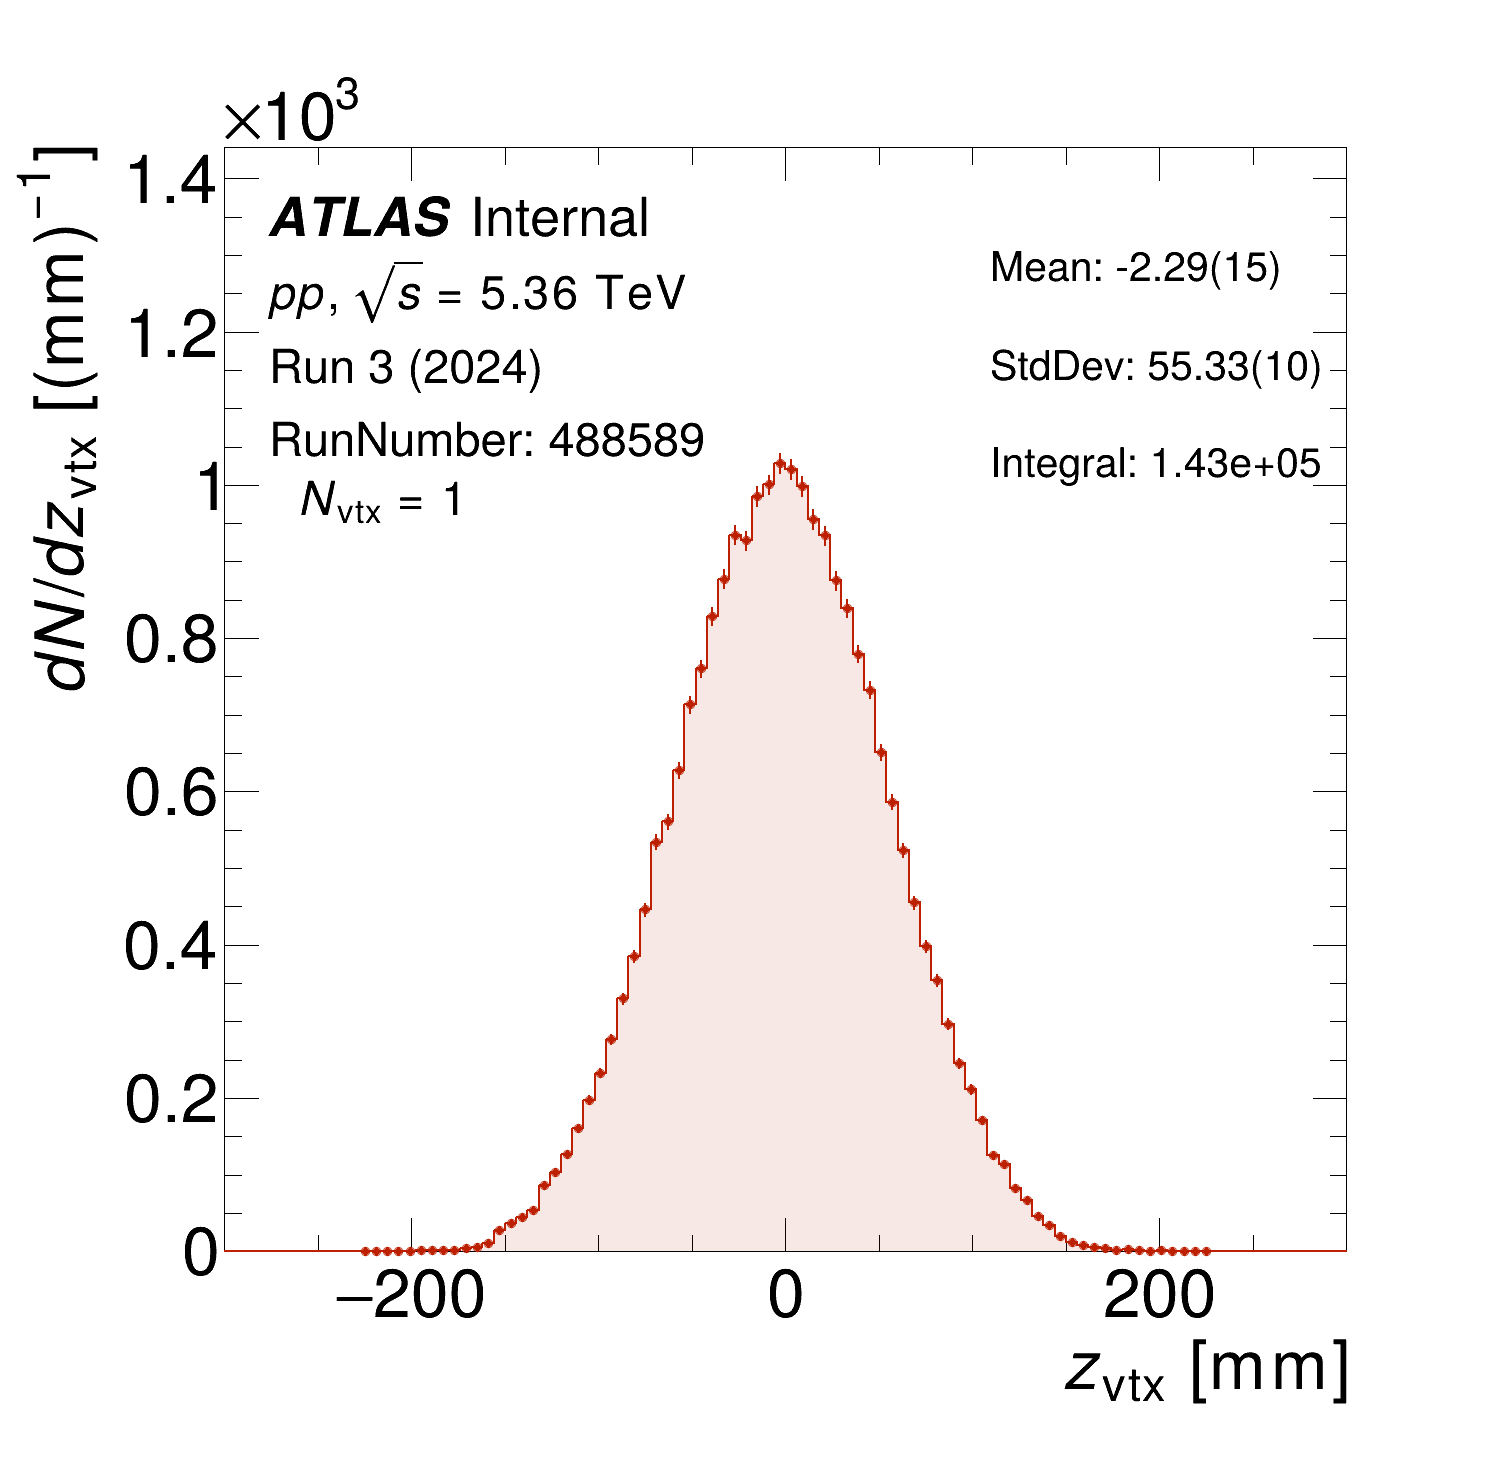
\includegraphics[width=0.45\linewidth]{images/vertex_z_488589.png}
      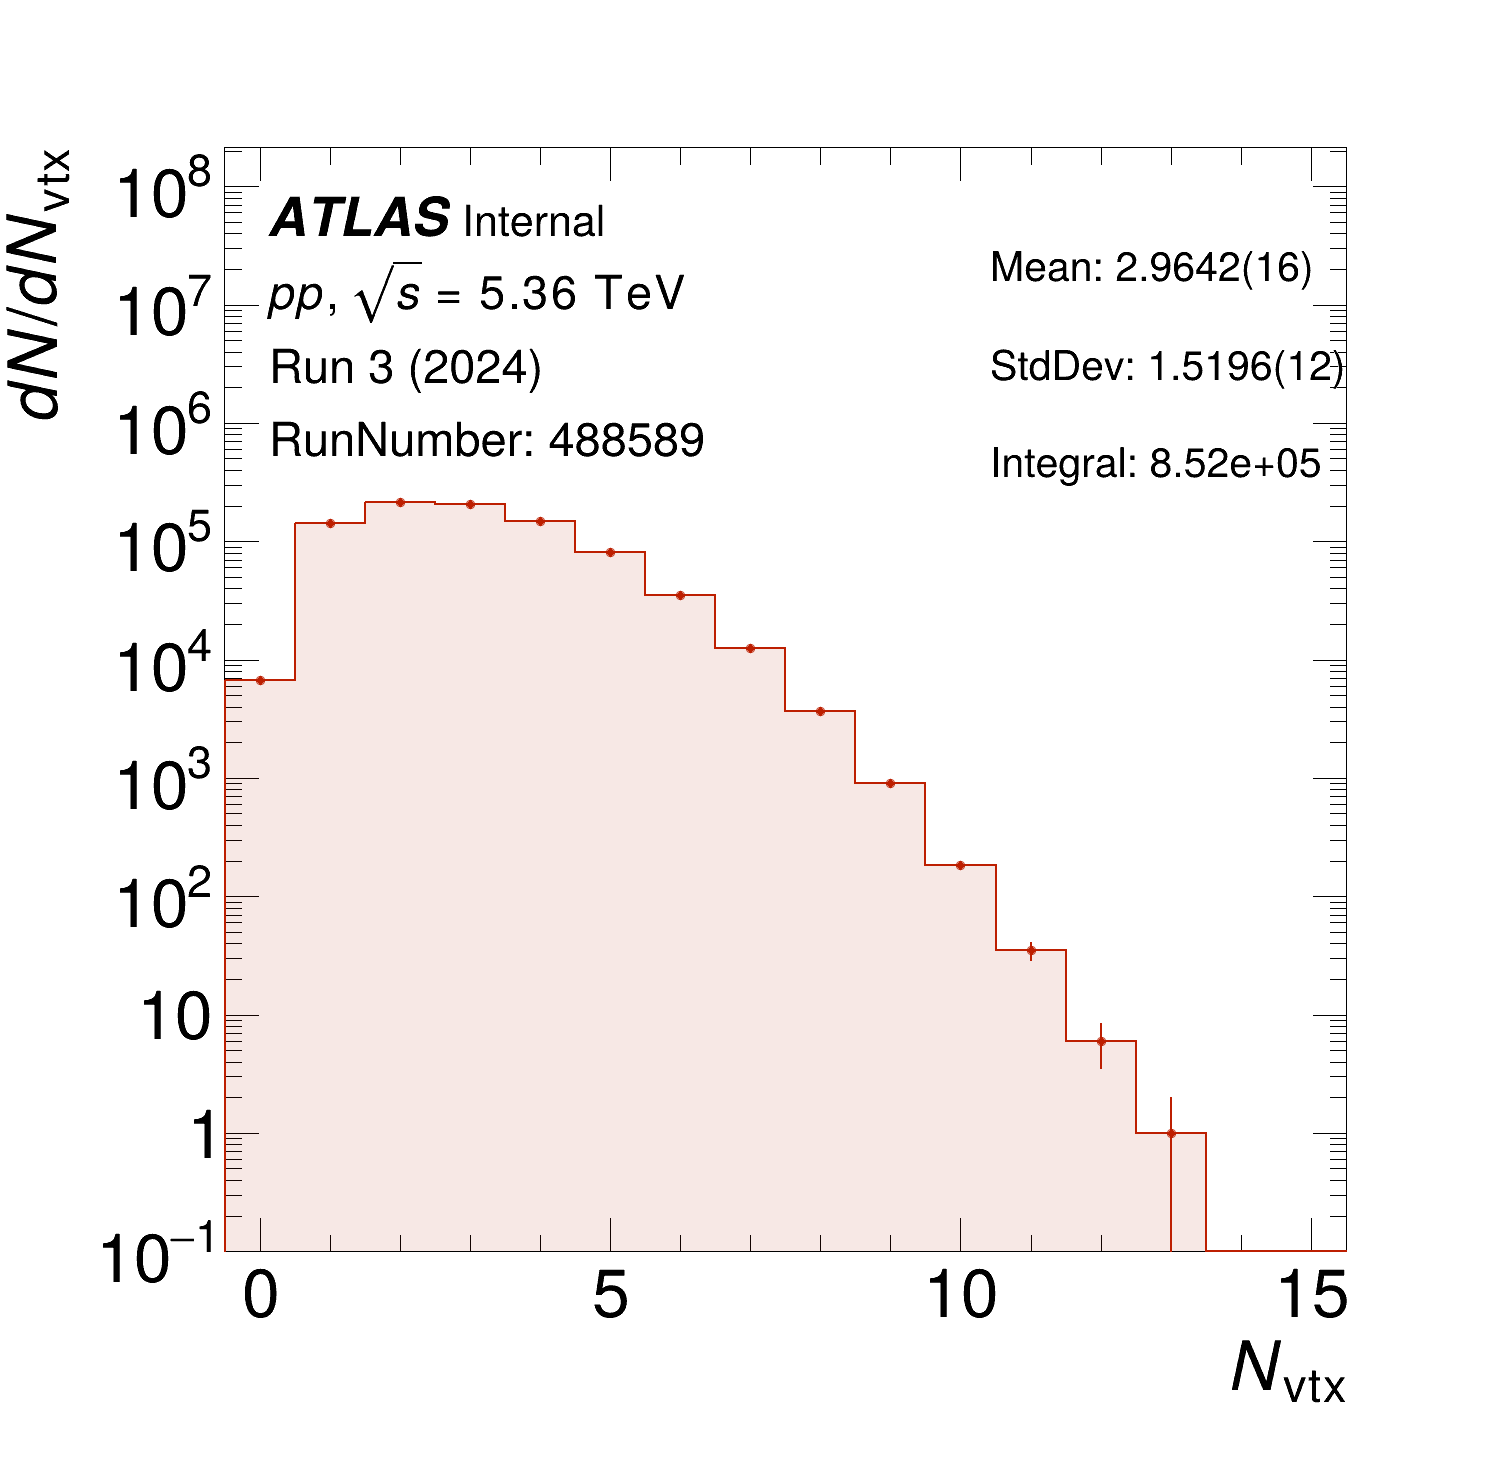
\includegraphics[width=0.45\linewidth]{images/nvertex_488589.png}
      \caption{Left: \zvtx distribution for events with $\nvtx=1$ in run 488589. Right: $\nvtx$ distribution in the same run.}
      \label{fig:nvtx_ppref}
  \end{figure}
The right panel of the same figure shows the number of reconstructed vertices found in the data. The $\langle \nvtx \rangle=2.96$ corresponds to $\mu\approx4$ in this run. This distribution is close to a Poisson, but it falls faster at high $\nvtx$ because the vertex merging depends on the number of collisions in a bunch crossing. 

To estimate this effect, the $\nvtx$ distribution was randomly generated assuming a Poisson shape for the number of vertices, and a Gaussian distribution in \zvtx. The width of the Gaussian is chosen the same as shown in the Figure~\ref{fig:nvtx_ppref}, and the mean value of generated vertices is slightly above the mean value in the Figure. Using the merging probability function shown in the right panel of Figure~\ref{fig:vtx_z_dist}, the number of vertices was recalculated. 
%According to this distribution, $N_\text{gen}^{\text{truth}}$ vertices are sampled. The number of vertices to be generated is sampled from a Poisson distribution with $\lambda$ taken as $\langle \nvtx \rangle=2.96$ from $\pprefSample$ data (see fig.~\ref{fig:nvtx_ppref}). 
The generated number of vertices is tuned iteratively to match the generated distribution after merging to the real data distribution up to a percent accuracy in the region of $\nvtx \leq 8$ %(see %fig.~\ref{fig:ratio_nvtx_real_over_fake}). 
The ratio of recalculated to measured $\nvtx$ is shown in Figure~\ref{fig:ratio_nvtx_real_over_fake}.
  \begin{figure}[h]
      \centering
      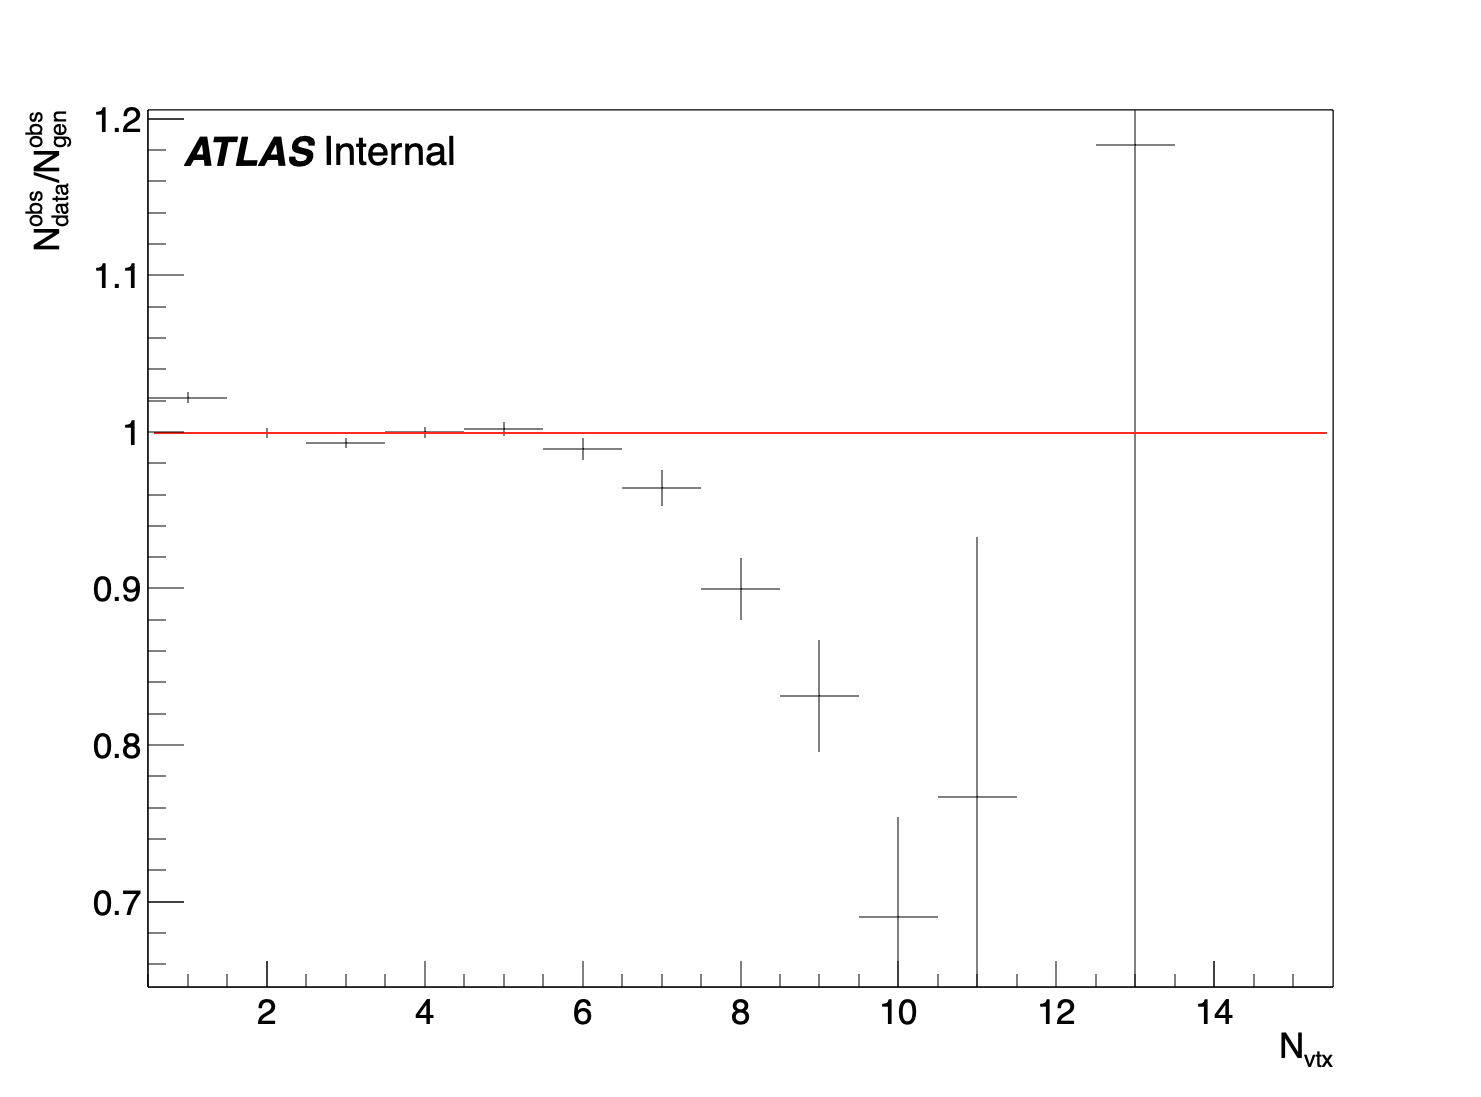
\includegraphics[width=0.5\linewidth]{images/nvtx_gen_real.png}
      \caption{Ratio of real $\nvtx$ distribution to $N_\text{gen}^\text{obs}$}
      \label{fig:ratio_nvtx_real_over_fake}
  \end{figure}
The region of $\nvtx > 8$ deviates from unity, however it contains less than $0.5\%$ of analyzed events.

Vertex merging was implemented in two different flavors. A simple merging algorithm orders the vertices in $z$ and merges them based on the probability explained above. The merging is performed sequentially, and when the two vertices are merged, they are replaced by a single vertex in the middle. The algorithm stops when the last vertex in $z$ is reached. A clustered merging algorithm starts with a vector of vertices, producing a binary merging decision for each pair of neighboring vertices, giving rise to a vector of boolean decisions: true or false. If there are $n$ consequential 'true' evaluations, corresponding $n$+1 vertices are merged into one located at the center of mass of these $n$+1 vertices. No significant difference was observed between these two approaches. %(see appendix, fig.~\ref{fig:ratio_seq_clus_merger}). {\red if there is no difference, I'd not invent an appendix for it}

After running the merging algorithm, the number of observed vertices is counted $N_\text{gen}^\text{obs}$. A map between the observed number $N_\text{gen}^\text{obs}$ and the truth number of vertices before merging $N_\text{gen}^\text{truth}$ is constructed shown in  Figure~\ref{fig:nobs_vs_ngen}.
  \begin{figure}[h]
      \centering
      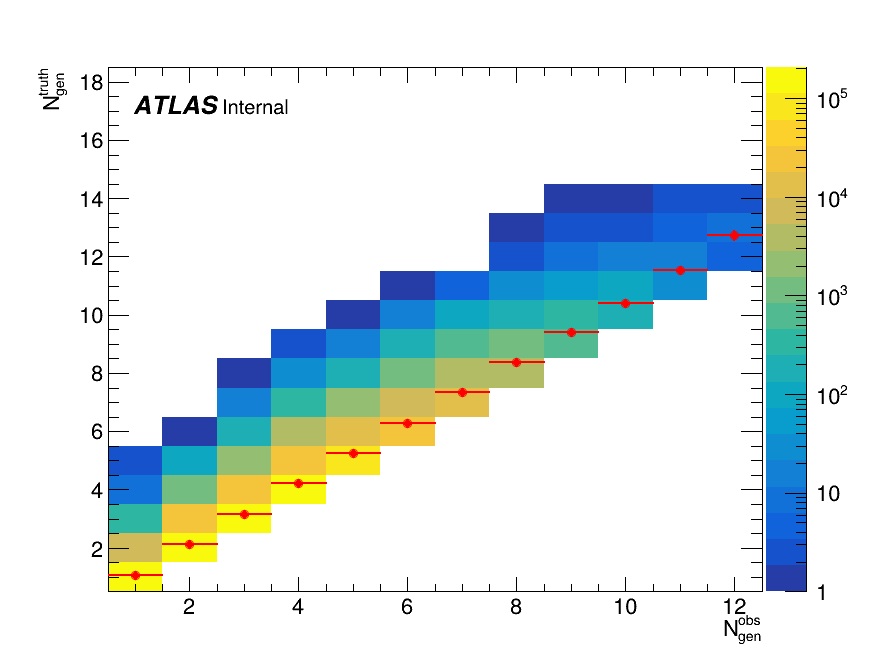
\includegraphics[width=0.45\linewidth]{images/nobs_vs_ngen.png}
      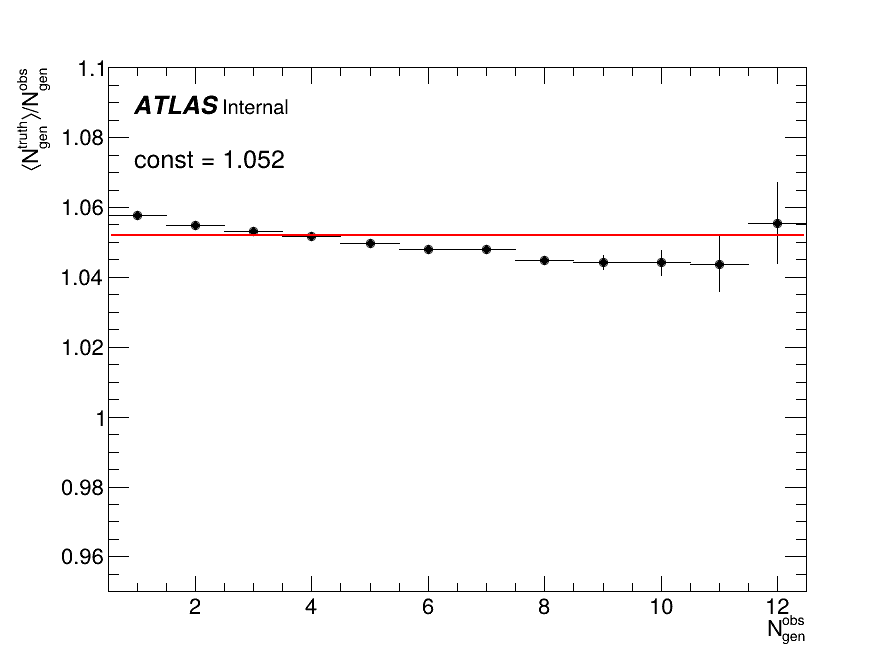
\includegraphics[width=0.45\linewidth]{images/ratio_nobs_ngen.png}
      \caption{Left: 2D distribution of $N_\text{gen}^\text{obs}$ vs $N_\text{gen}^\text{truth}$. Right: correction factor $\varepsilon_\text{m} (N_\text{gen}^\text{obs})$}
      \label{fig:nobs_vs_ngen}
  \end{figure}
  
  For each $N_\text{gen}^\text{obs}$ $\langle N_\text{gen}^\text{truth}\rangle$ is calculated. Then, a correction factor to adjust for merging is defined as 
  \begin{equation}
      \varepsilon_\text{m}(N_\text{gen}^\text{obs}) =\langle N_\text{gen}^\text{truth}\rangle/ N_\text{gen}^\text{obs}
  \end{equation}
  The total correction factor is taken as average over $N_\text{gen}^\text{obs}$
  \begin{equation}
      \varepsilon_\text{m} = \sum_{N_\text{gen}^\text{obs}} p(N_\text{gen}^\text{obs})\varepsilon_\text{m}(N_\text{gen}^\text{obs})
  \end{equation}
and equal to 1.052 in $\langle \mu \rangle \sim 4.0$ data. {\blue To be updated -- calculated as a function of $\mu$.} 

% {\red a logical end to this section would be Figure~\ref{fig:tpvreco_bothmu}, and discussion of $N_{\mathrm{evt}}$ correction followed by the discussion of $\omega$ cuts, see my text around that figure. But to do it right, the first thing is to work out the correction not for a single $\mu$ but for any $\mu$ up to say $\mu$ of 5 and plot it as a curve.}
  
\section{Correction for track acceptance difference between 2024 and 2025 conditions}
{\blue Will be determined by comparing full-sim Pythia MCs with $\pprefSample$ and before-$\OO$ conditions.}

\section{Correction of $\avgNcoll$}
Although the \Ncoll needed for \RAA is extracted from the Glauber model, one shall take into account that the MinBias sample is not fully inclusive, and some losses are anticipated for events with low multiplicity.
{\blue Will be determined when $\OO$ data is available.}
% {\red why does one need oxygen data for that? one can do it by convolving \pp. Generally, I think this  discussion should go to \Ncoll calculations using Glauber}



\section{Correction for transmutation}\label{sec:transmutation_correction}

If oxygen dissociates into lighter nuclei with the same rigidity ($A/Z$), these lighter ions could stay circulating in the beamline together with oxygen \cite{transmutation_lpc}. The dissociation can be caused by electromagnetic dissociation or by hadronic fragmentation processes. Certain theoretical models describing oxygen as a cluster of 4 \al particles give an exceptionally high cross section to the hadronic fragmentation in \al particles, causing contamination of the \OO collisions with \Oa and \alal collisions with increasing time of the beam circulation. Such contamination (if significant enough) would inevitably affect the measurement of $\RAA$.

The approach to mitigate a possible contamination is to select the fragment of data with lower contamination levels, and by the level of contamination to increase the systematic on $\avgNcoll$ or adjust $\avgNcoll$ as a function of the contamination. Thus, one needs to be able to estimate the fraction of \Oa and \alal in the data. Assuming the average number of tracks per collision (vertex) $\tpv$ (see below) is constant, as it originates in the type of collided system and reconstruction efficiency, one can study this variable during the \OO data-taking to constrain the contamination of \OO by \Oa (\alal). One also assumes the collisions start with a pure \OO sample and the contamination builds up over time, leading to a decrease in $\tpv$, which can serve as a proxy for the contamination.


% editing stop here -> check nchar vs. ntrk in Hijing and Angantyr... we have full reco now

Using HIJING simulations for the \OO and \Oa collisions, histograms for the number of charged hadrons $\nchar$ with $|\eta|< 2.5$  and $\Npart$ were populated. Additionally, $\Npart$ and $\ntrk$ were simulated in Angantyr and Glauber. Sampling from these histograms based on the probability of the $\OO$ and $\Oa$ collisions (see below), histograms of gradually growing contamination were created. The rate of collisions of various species can be determined as: 

\begin{equation}
\begin{split}
    p_{\OO} = f_{\mathrm{O}}^{2} \sigma_{\OO} \mathcal{L}, \\
    p_{\Oa} = 2 f_{\mathrm{O}} f_{\alpha} \sigma_{\Oa} \mathcal{L}, \\
    p_{\alal} = f_{\alpha}^{2} \sigma_{\alal} \mathcal{L},
\end{split}
\end{equation}
where $f_{\mathrm{O}}$ is the fraction of oxygen nuclei in the beams, $\mathcal{L}$ the instantaneous luminosity, and $f_{\alpha}$ is the fraction of $\alpha$. Given $\alpha$ is expected to play the dominant role among the parasitic nuclei species in the \OO beam, we set for simplicity $f_{\mathrm{O}}$+$f_{\alpha} = 1$. Corresponding cross-sections $\sigma_{\OO}= (1.33\pm0.07)$~b, $\sigma_{\Oa} = (0.71\pm0.02$)~b, and $\sigma_{\alal} = (0.328\pm0.002)$~b have been obtained from the MC Glauber simulations and may have limited precision. Having these probabilities at hand, one can study the ratio of events produced in $\Oa$ and $\alal$ collisions normalized to the number of $\OO$ collisions:
\begin{eqnarray}
\frac{p_{\Oa}}{p_{\OO}} &=& 2 \frac{f_{\alpha}}{(1-f_{\alpha})} \frac{\sigma_{\mathrm{\Oa}}}{\sigma_{\mathrm{OO}}}, \nonumber \\
\frac{p_{\mathrm{\alpha\alpha}}}{p_{\mathrm{OO}}} &=& \frac{f^2_{\mathrm{\alpha}}}{(1-f_{\alpha})^2} \frac{\sigma_{\mathrm{\alpha\alpha}}}{\sigma_{\mathrm{OO}}} = 
\frac{1}{2}\frac{f_{\mathrm{\alpha}}}{(1-f_{\alpha})}
\frac{\sigma_{\alal}}{\sigma_{\alpha\mathrm{O}}}
\frac{p_{\Oa}}{p_{\OO}}.
\label{eqn:paa}
\end{eqnarray}
If the $\frac{p_{\Oa}}{p_{\OO}}$ contamination in the data stays within 20\%, the addition of \alal collisions in the data should not exceed 0.9\% using equations~\ref{eqn:paa}. Since the data collection limit is set to not exceed 10 \% $\alpha$ contamination, only $\Oa$ collisions are considered as a possible addition to \OO collisions.

Finally, the mean of the $\Npart$ and $\ntrk$ histograms was calculated. The means obtained normalized to the initial values of pure oxygen $\Npart(t=0)$ and $\ntrk(t=0)$ are shown as a function of $\frac{p_{\mathrm{\Oa}}}{p_{\mathrm{OO}}}$ in Figure~\ref{fig:corr_norm}. Normalization to the initial values is beneficial, as it removes the dependence on the detector effects. 

\begin{figure}[h]
    \centering    
    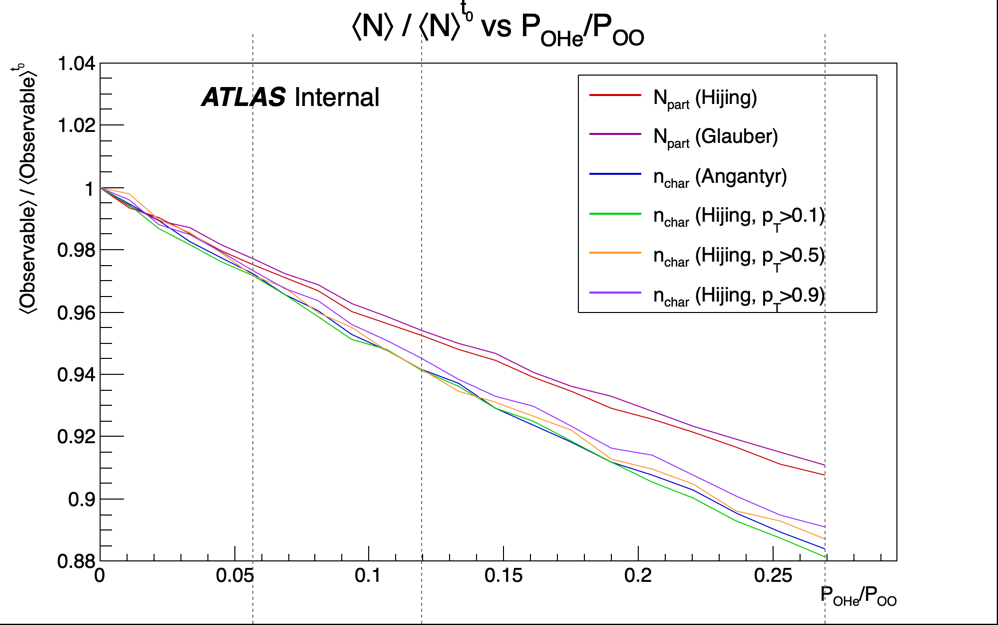
\includegraphics[width=\linewidth]{images/mixing_scan_all_observables.png}
    \caption{Average of $\Npart$ and $\ntrk$ normalized on the pure oxygen values as a function of the ratio between the probability (number) of parasitic and target events. Vertical dashed lines correspond to 5, 10, and 20 \% of $f_{\mathrm{\alpha}}$ beam contamination}
    \label{fig:corr_norm}
\end{figure}

One can see in Figure~\ref{fig:corr_norm} the difference between $\Npart$ and $\ntrk$ scaling, which requires further investigation. The difference between $\Npart$ and $\ntrk$ scaling should be considered a systematic error. Fortunately, the discrepancy is smaller for smaller values of $f_{\mathrm{\alpha}}$. Another feature of the $\Oa$ collisions is that the produced particles are boosted and $\OO$ are not. In $\OO$ HIJING used, a small asymmetry of the $\eta$ distribution of the charge particles (cut on the reconstruction and acceptance limit of the ATLAS - $\pT$ > 0.1, |$\eta$| < 2.5) was observed, as shown in Figure~\ref{fig:eta_ntrk}. This phenomenon requires further investigation. 
\begin{figure}[h]
    \centering
    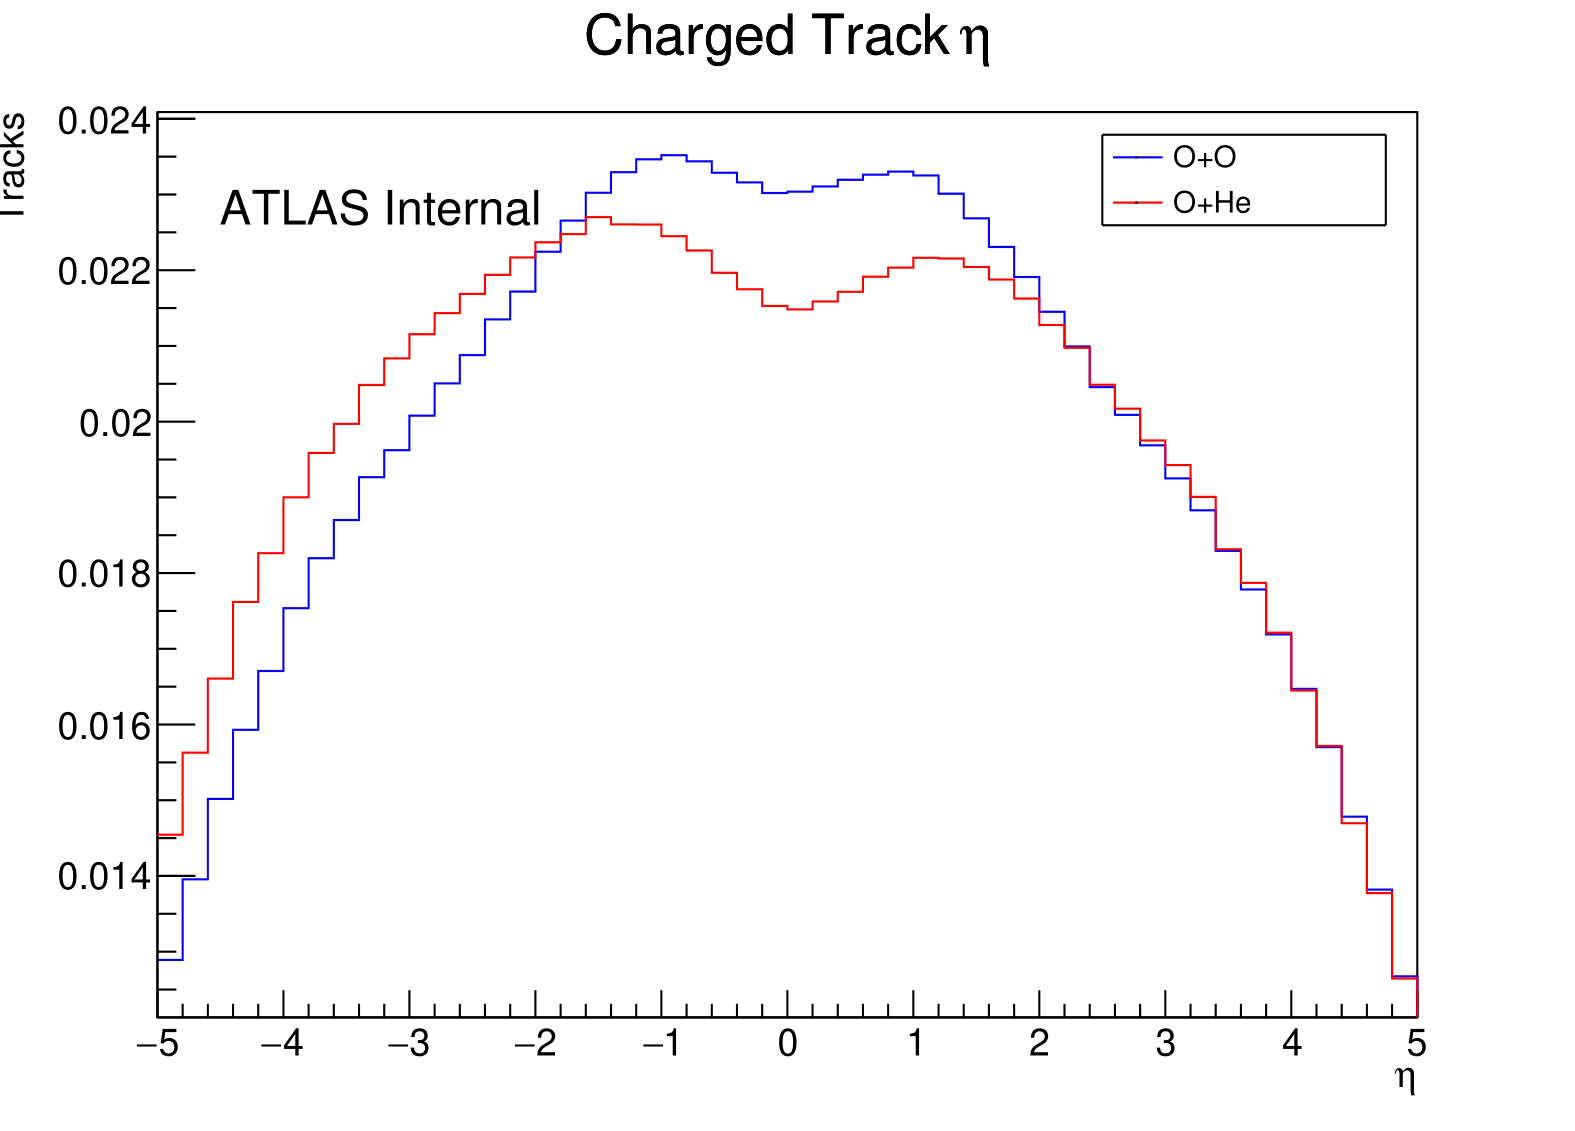
\includegraphics[width=\linewidth]{images/eta_comparison.png}
    \caption{$\eta$ distribution of charged particles in HIJING $\OO$ and $\Oa$ (normalized on the integral), one can see the boosted distribution in $\Oa$ collisions and the so far not understood asymmetry in $\OO$ collisions.}
    \label{fig:eta_ntrk}
\end{figure}

Critical for the measurement in case of the transmutation is the ability to measure the $\frac{p_{\mathrm{\Oa}}}{p_{\mathrm{OO}}}$ based on the drop of the $\tpv$, which allows us to adjust $\Ncoll$ to reflect on the admixture of helium in the collision system.

For the success of the method, it is also needed to adjust for the drop of $\tpv$ originating in the dropping $\mu$, and accordingly, the $\tpv$ should not change for one collision system without the change of $\mu$. As a hint to understand the stability of the average number of tracks per vertex
$\tpv$ was considered:
\begin{equation}
  \tpv = \langle \ntrk^\text{sel}(\text{vtx}_i) \rangle,
\end{equation}
where $\ntrk^\text{sel}(\text{vtx}_i)$ is the number of selected tracks that pass the following criteria:
\begin{enumerate}
    \item Quality: TightPrimary 
    % {\red \pT, $\eta$? why shall it be different from section 4?}
    \item Matched to vertex $i$ based on cuts on $d_0$ and $\omega_0$:
    \begin{equation}
        |d_0| < \qty{1.5}{\mm}, \quad
        |\omega_0| < \qty{1.5}{\mm}, \quad
        |d_0/\sigma_{d_0}| < 4, \quad
        |\omega_0/\sigma_{\omega_0}| < 4.
    \end{equation}
\end{enumerate}
One can notice that these are the track final selections without the track-to-vertex and the track-to-jet matching criteria. $\tpv$ was studied in the $\pprefSample$ sample as a function of $\mu$, vertex position $\mathrm{z_{vtx}}$, and LB number representing the temporal dependence. See Figure~\ref{fig:highmu_lowmu_tpv} for these dependencies in high-$\mu$ and low-$\mu$ samples. 
%{\red What am I supposed to learn from these six colorful plots? A good way to decide whether you need a plot or not (and whether it is plotted correctly) is to ask yourself if you can derive any conclusion from the plot that helps the flow of convincing the reader that you are doing the right things, i.e., explaining the analysis. If not, then the plot is not needed.} Agreed, will be removed when new set of plots presented

A mild increase of $\tpv$ is seen with increasing $\mu$ (when $\mu \sim 4$), which is attributed to the effect of vertex merging (see Section~\ref{sec:vertex_merging}), since a merged vertex must have more tracks, thus moving the mean. 
%The same effect is seen on $z_\text{vtx}$ distribution ($\mu\sim 4$), where the maximum $\tpv$ is reached towards the center of the distribution, where again merging of vertices is dominant (simply because the vertex "density" there is larger).

\begin{figure}[h]
    \centering
    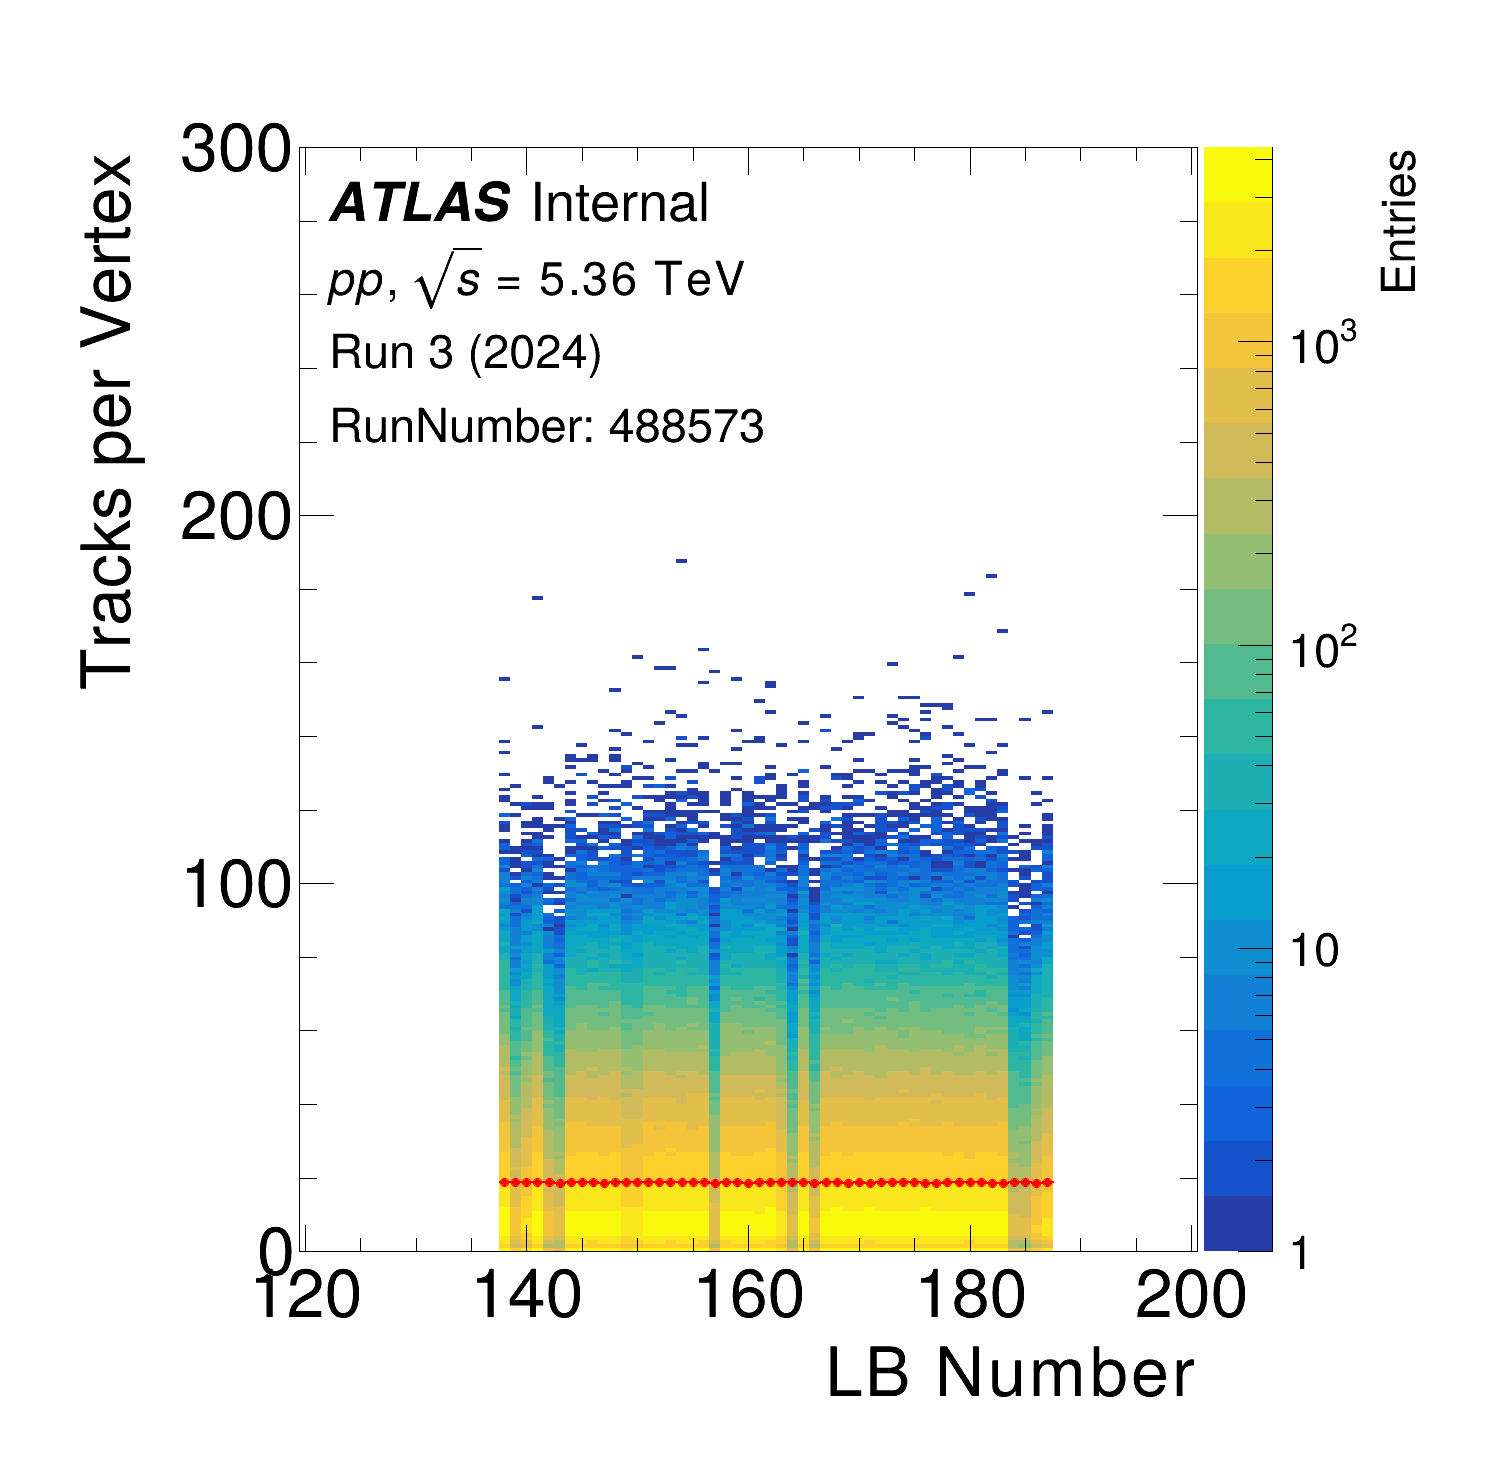
\includegraphics[width=0.32\linewidth]{images/tpv_lb_high_h2d_tpv_lb_488573.png}
    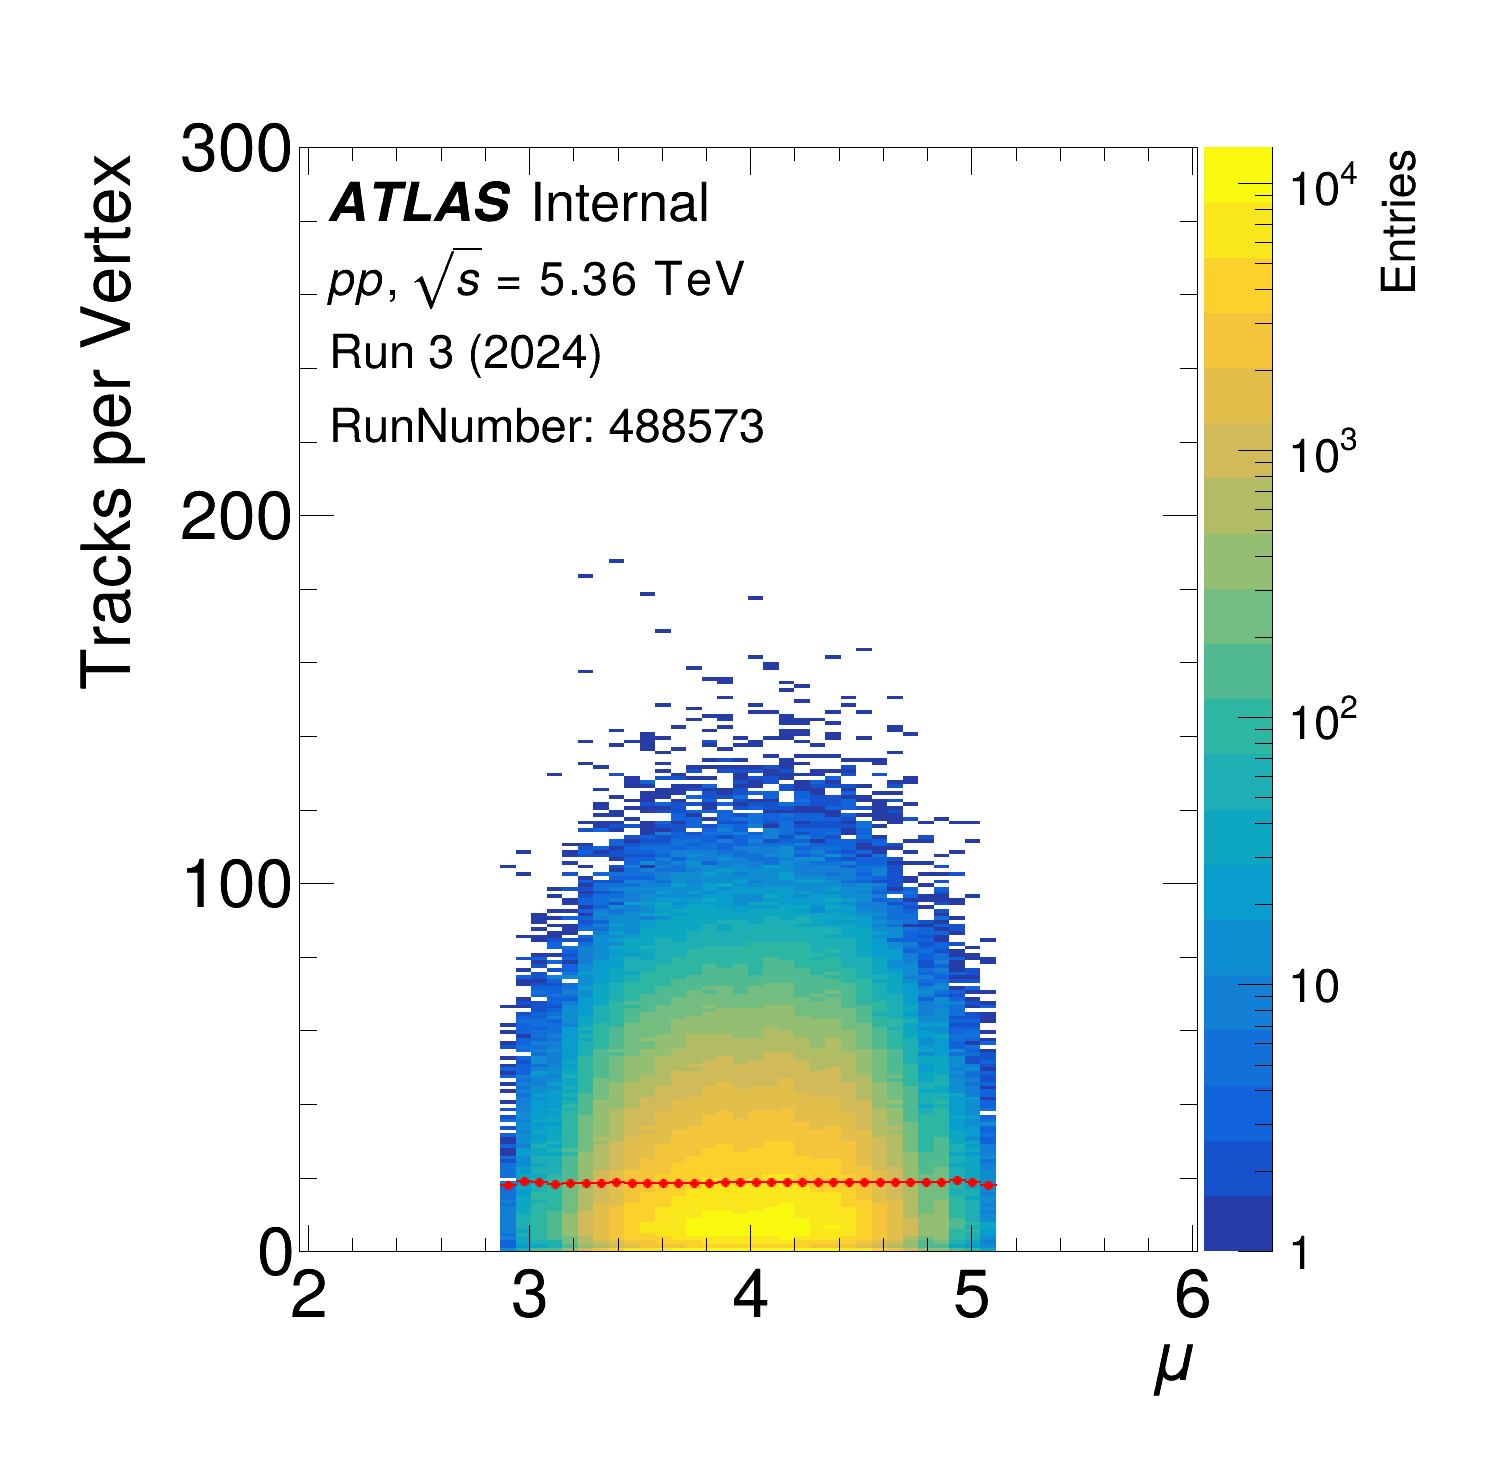
\includegraphics[width=0.32\linewidth]{images/tpv_mu_high_h2d_tpv_mu_488573.png}
    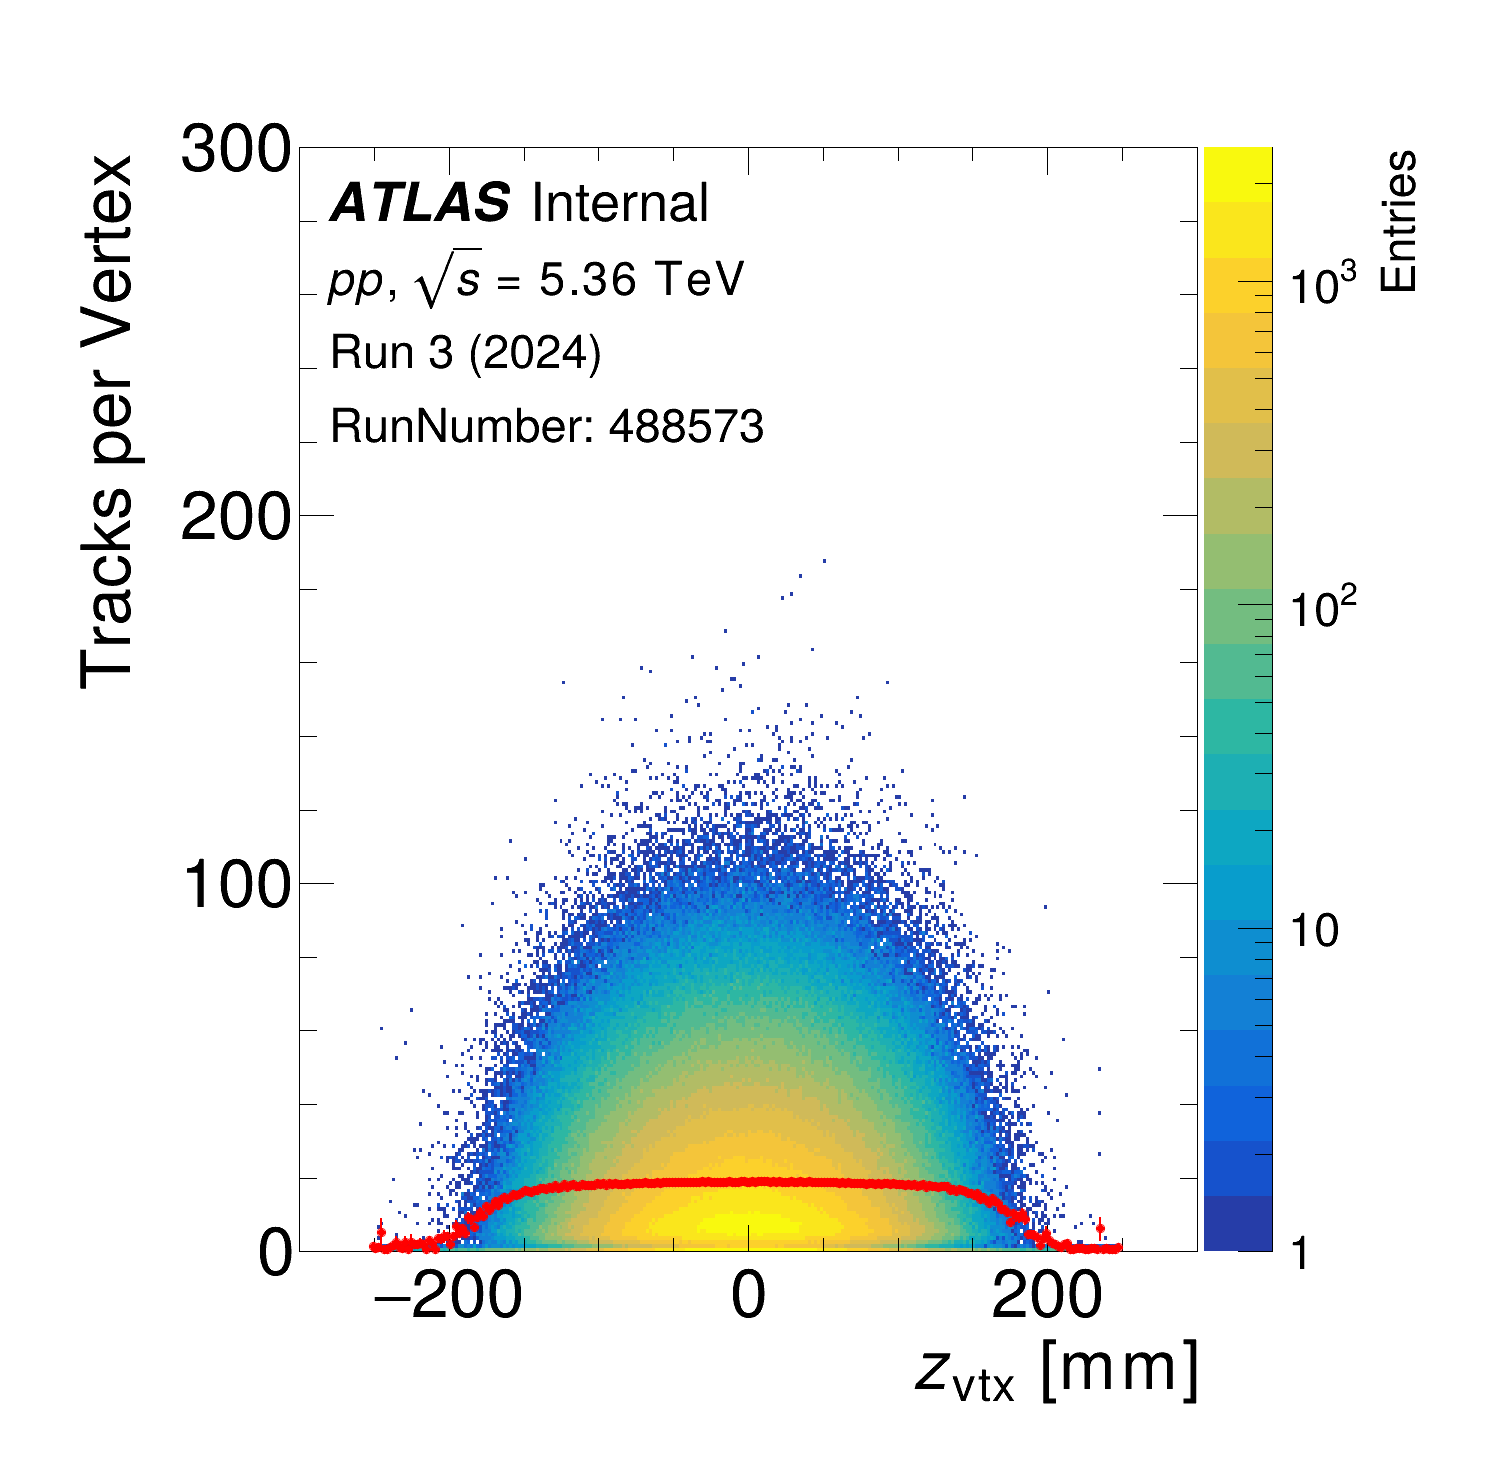
\includegraphics[width=0.32\linewidth]{images/tpv_zvtx_high_h2d_tpv_zvtx_488573.png}
    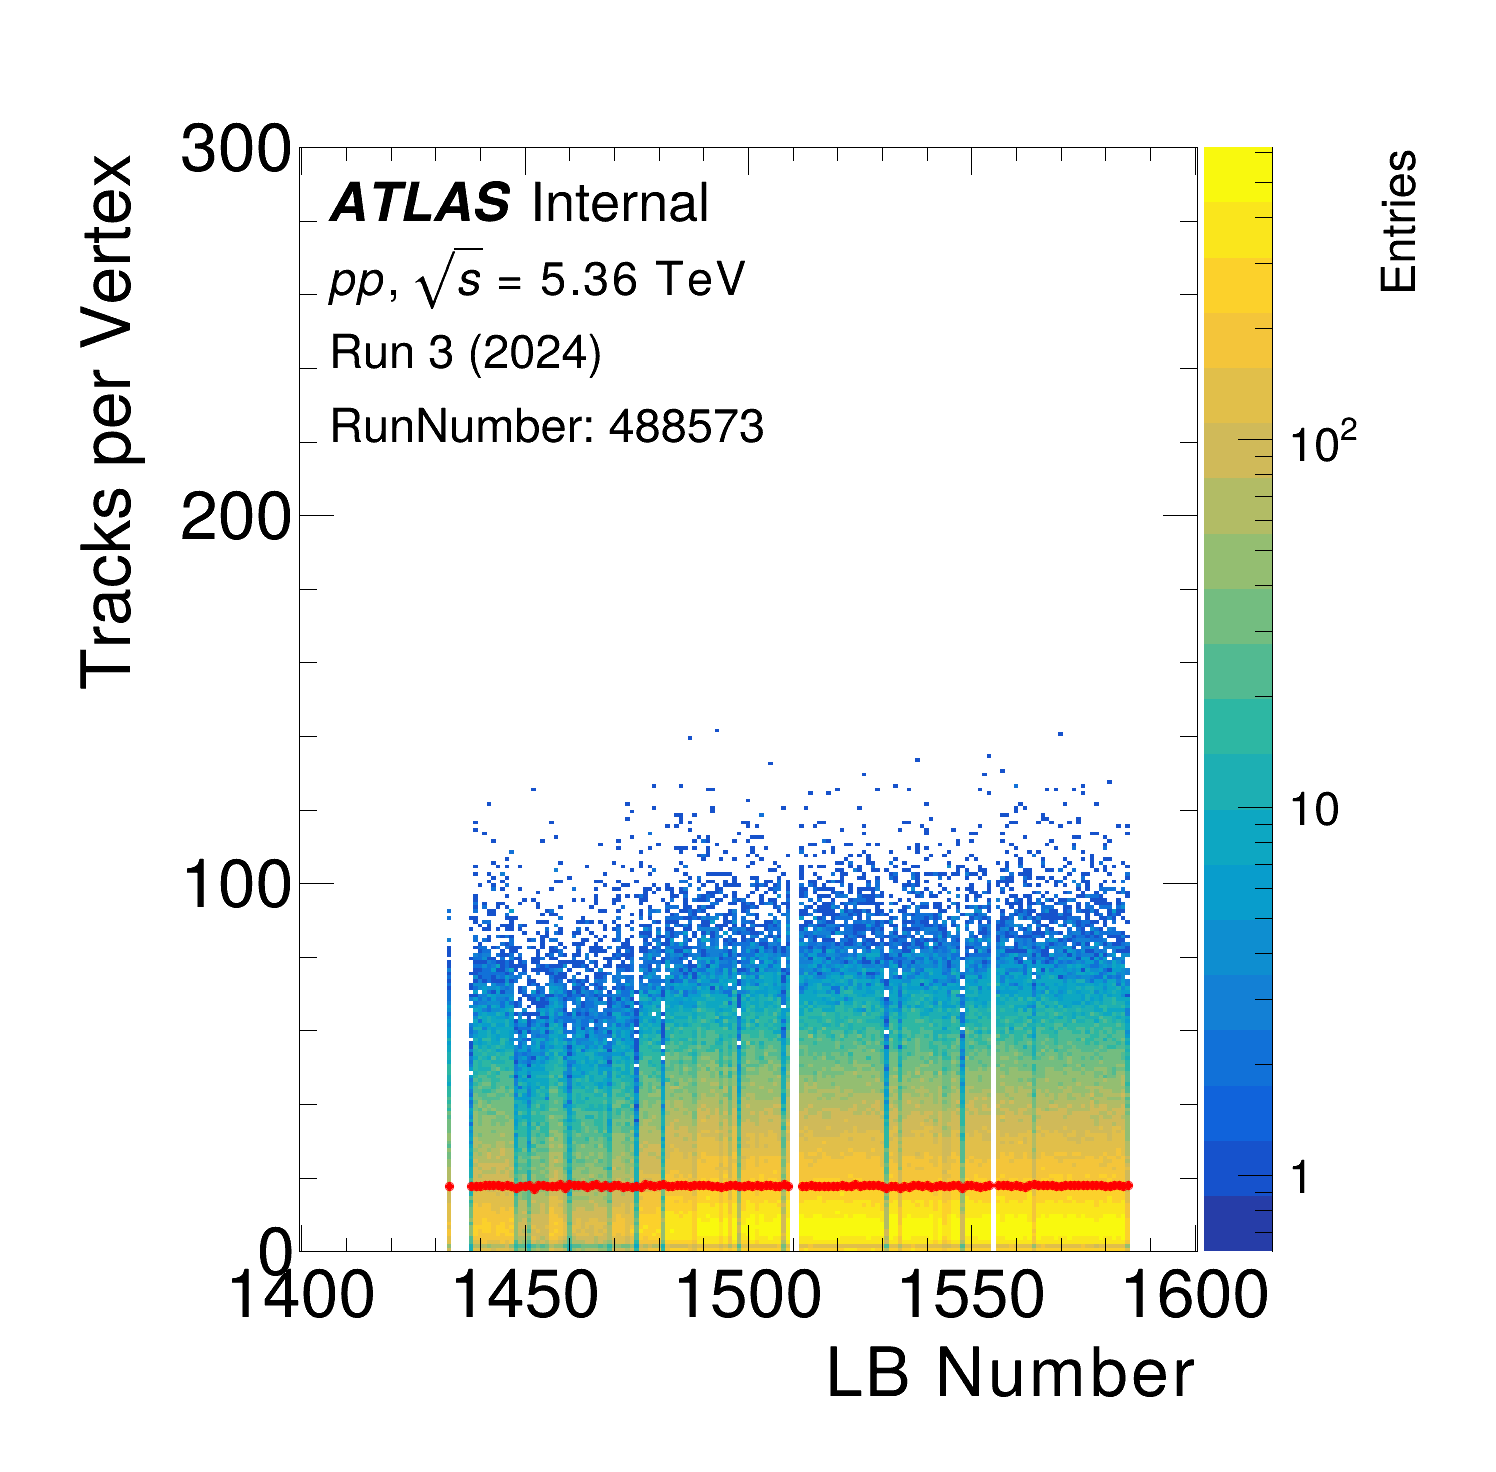
\includegraphics[width=0.32\linewidth]{images/tpv_lb_low_h2d_tpv_lb_488573.png}
    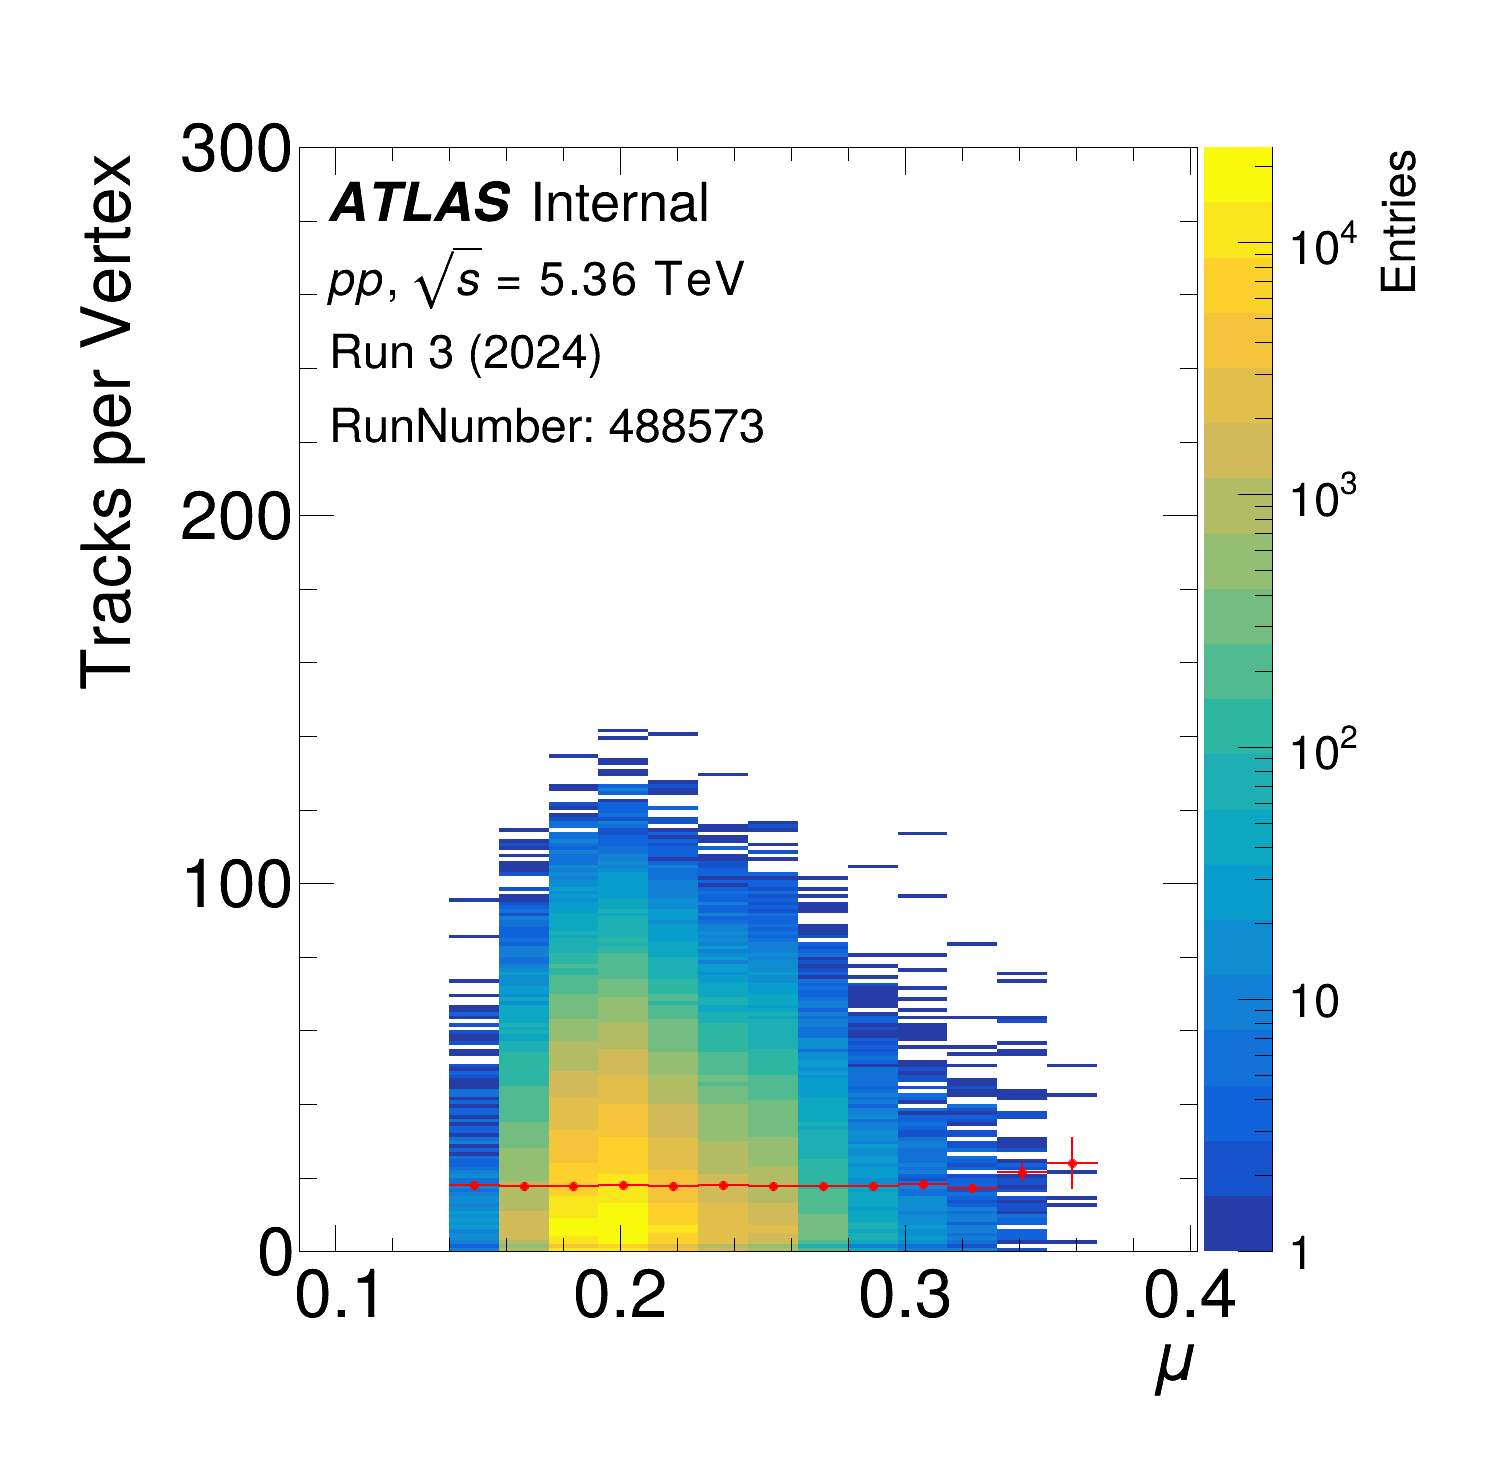
\includegraphics[width=0.32\linewidth]{images/tpv_mu_low_h2d_tpv_mu_488573.png}
    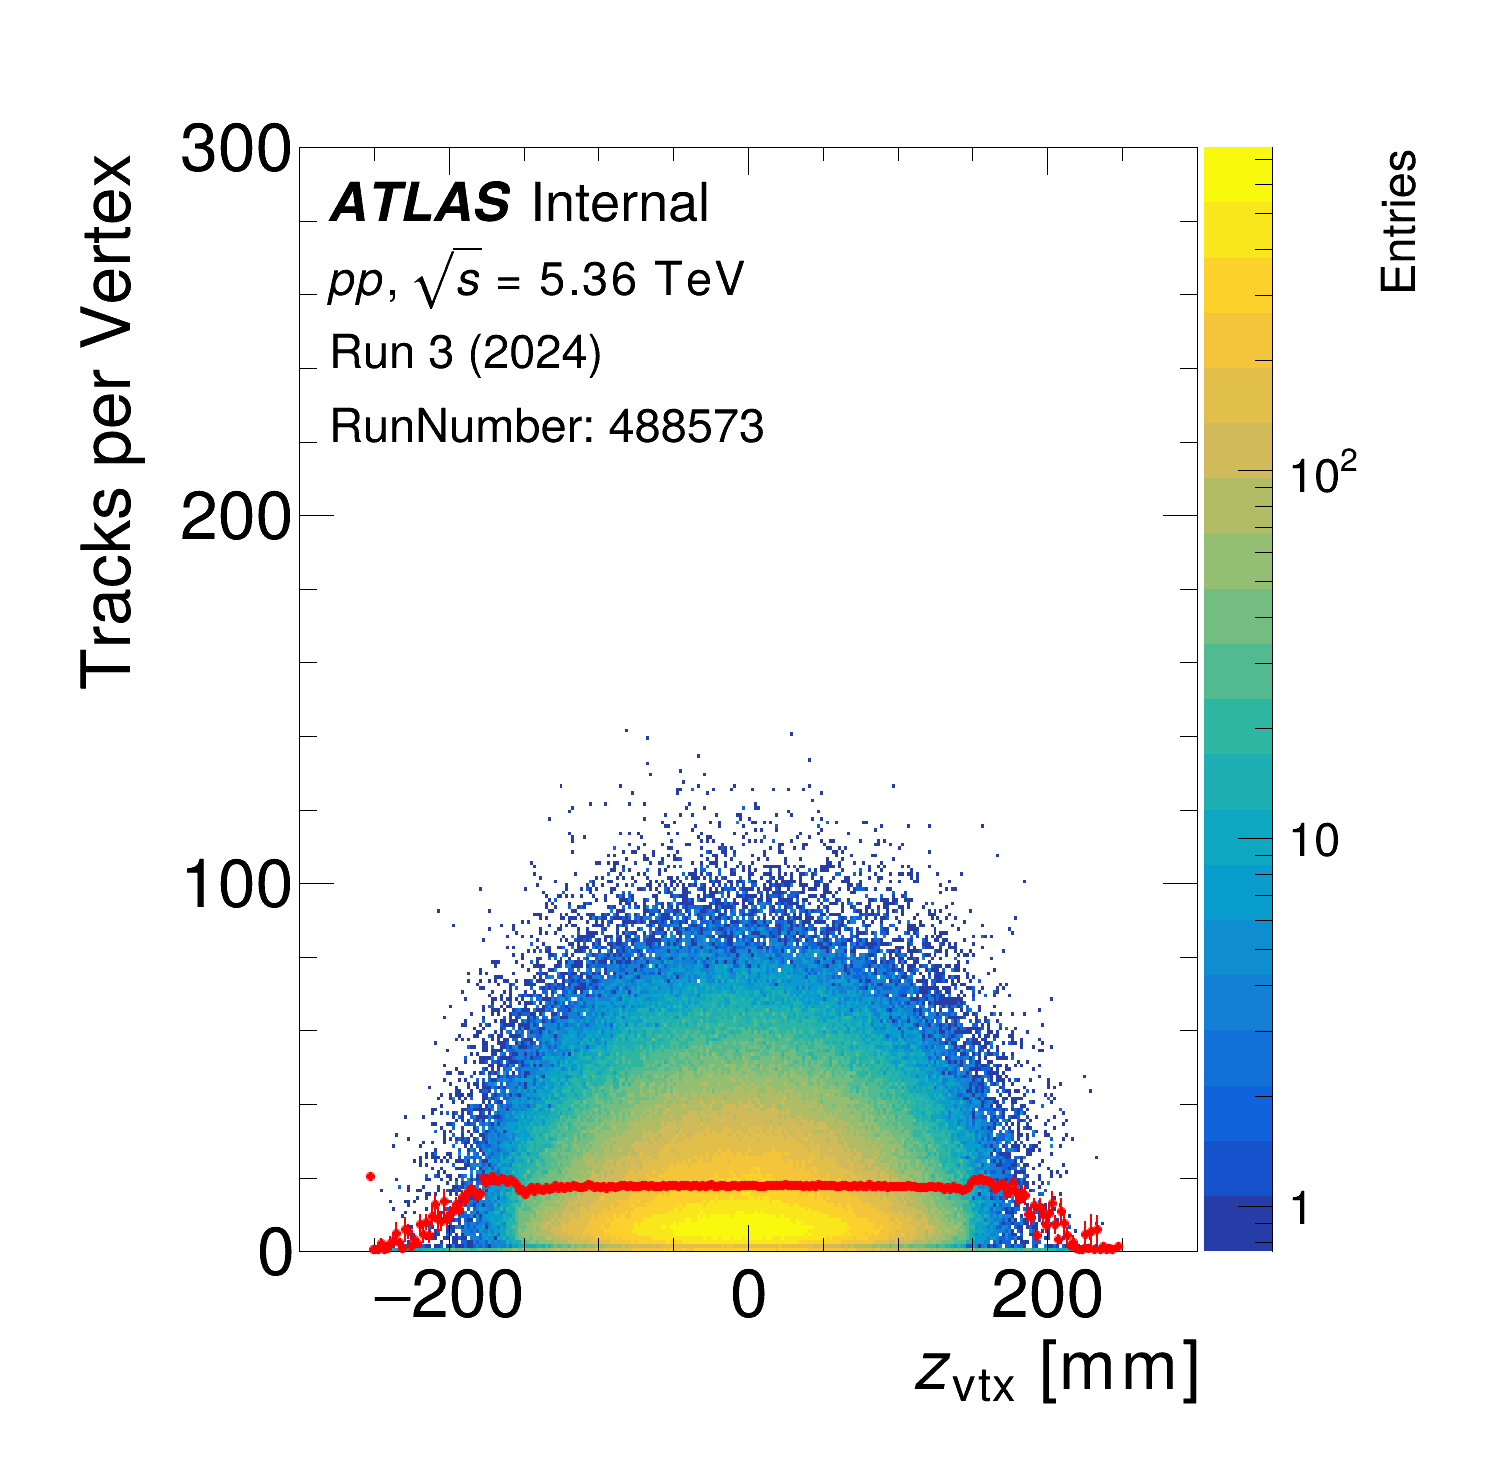
\includegraphics[width=0.32\linewidth]{images/tpv_zvtx_low_h2d_tpv_zvtx_488573.png}
    \caption{$\tpv$ distributions in high-$\mu$ (top row) and low-$\mu$ (bottom row) samples. Left: as a function of lumiblock number. Middle: as a function of $\mu$. Right: as a function of $z_\text{vtx}$.}
    \label{fig:highmu_lowmu_tpv}
\end{figure}

As $\OO$ mean $\mu$ is expected to be low ($\sim 0.3$), the $\tpv$ dependencies in $\pprefSample$ low-$\mu$ sample can be taken as reference. Less granular quantities can be defined
\begin{equation}
    \avgtpvreco = \frac{N_\text{trk}^\text{reco}}{N_\text{vtx}}, \quad 
    \avgtpvsel = \frac{N_\text{trk}^\text{sel}}{N_\text{vtx}}, \quad 
\end{equation}
where subscript $\text{reco}$ refers to reconstructed tracks (no selections applied) and $\text{sel}$ subscript refers to tracks selected as ''TightPrimary'' \&\& $|d_0|<\qty{1.5}{\mm}$ \&\& $|d_0/\sigma_{d_0}|<4$. 
%{\red already explained. when you repeat things in the text, you make them less certain to a reader. much better way is to define tracks once and always use the same tracks.} This is done here to emphasize not using omega0 cut... Will be reiterated
They are equivalent to $\tpv$ in the regime of low-$\mu$, as then $\nvtx \sim 1$. As can be seen from Figure~\ref{fig:tpvreco_bothmu}

% {\red Figure~\ref{fig:tpvreco_bothmu} belongs to the end of section 5.3, and it has to have 3 curves. To put them on one canvas, one can rebin $\mu$ intervals at the edges such that the error bars are not too large there, or just ignore points with error bars greater than 1/2 track (must be mentioned in the captions). 

% The first curve must be as shown. 

% The second curve must be after applying the correction explained in section 5.3. The anticipated effect is that the left interval will stay where it is, but the right interval will go significantly down, I would expect below 24-25 tracks. The correction must be applied differently for each value of $\mu$. 

% The third curve also must have the correction applied for vertex merging, but it should have a different track selection with $\omega$ cuts. For example, the first set of cuts should assign any track to the nearest vertex regardless of $\omega$, and the other set of cuts should use the full suite of $\omega$-based selection. The anticipated effect of the third curve is that it may go up or down depending on which set you use originally, but both $\mu$ intervals would become flat.

% Using the figure, we must make a conclusion that merging move vertices and invalidating the $\omega$ cuts, and deciding whether we shall or shall not use them at all. In here, you can simply refer to that plot in section 5.3}

% This will be added in the next version



\begin{figure}[h]
    \centering
    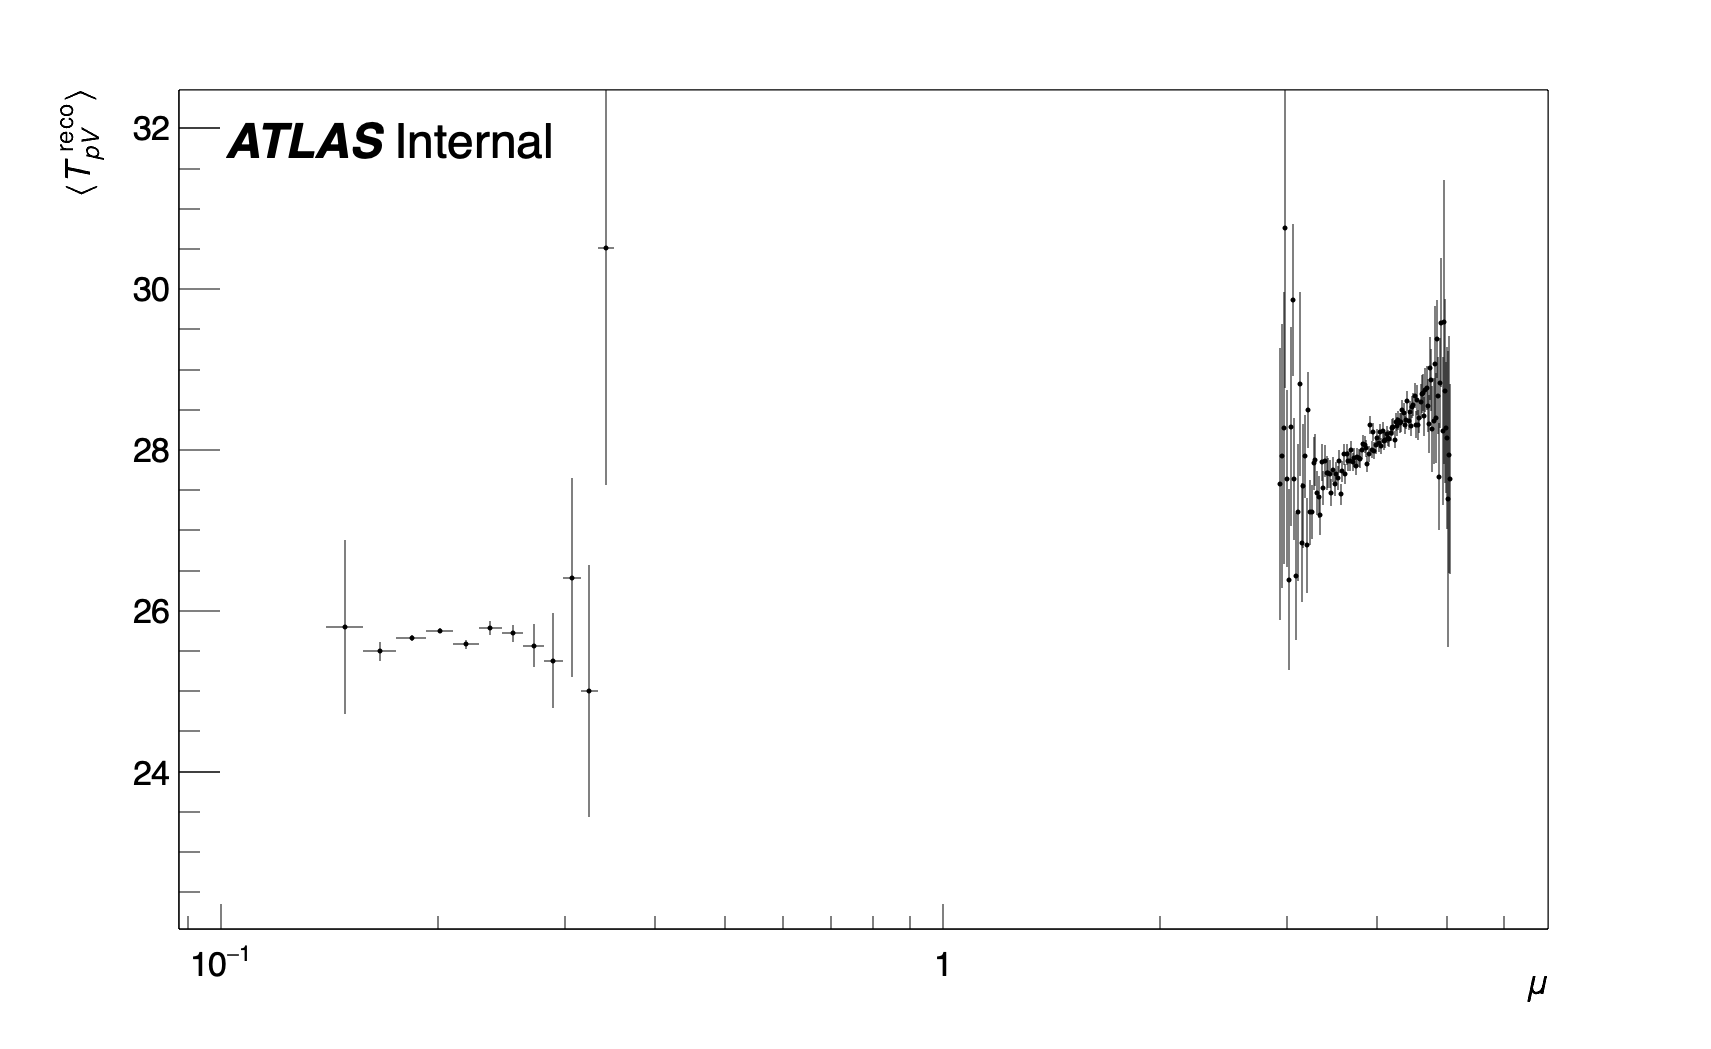
\includegraphics[width=1.0\linewidth]{images/TPVreco_bothmu.png}
    \caption{Dependence of $\langle \avgtpvreco \rangle$ on $\mu$ in chunk of $\pprefSample$ sample ($\langle \mu \rangle\sim 0.2$ and $\langle \mu\rangle\sim 4.0$)}
    \label{fig:tpvreco_bothmu}
\end{figure}
the quantity $\langle \avgtpvreco \rangle$ is constant in the regime of low-$\mu$, and is rising for high-$\mu$ (due to effect of merged vertices). 


%Distributions of $\tpv$ as a functions of lumiblock, $\mu$ and $z_\text{vtx}$ were fitted with pol1. Resulting slopes are consistent with 0 within $2\sigma$ with $\chi^2/\text{ndf}\sim 1$. Dependence on $z_\text{vtx}$ still have certain degree of a non-constant behavior in range $|z_\text{vtx}| > \qty{100}{\mm}$
% \begin{figure}[h]
%     \centering
%     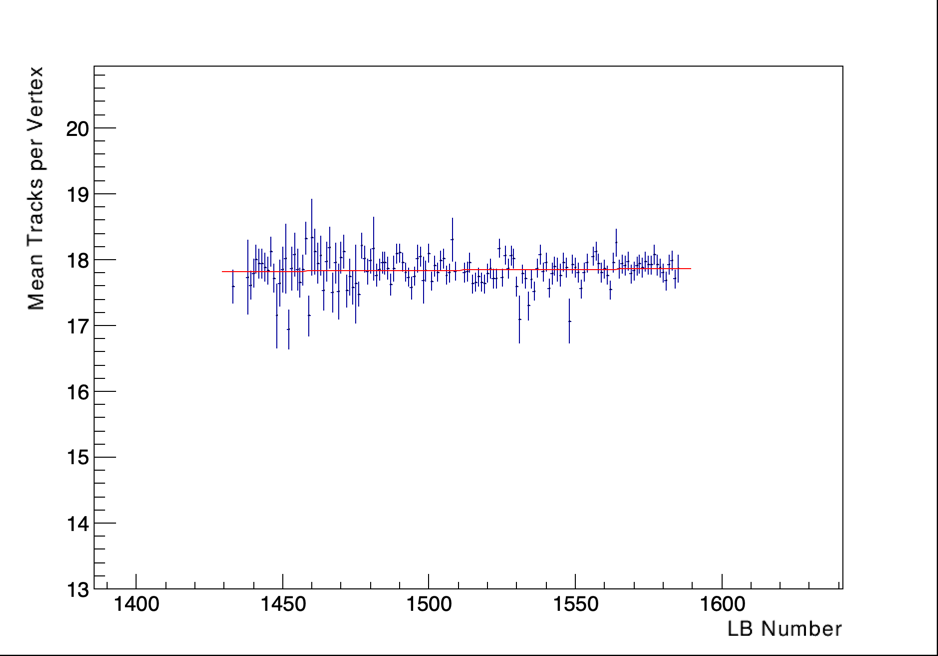
\includegraphics[width=0.32\linewidth]{images/meantpv_lowmu_lb.png}
%     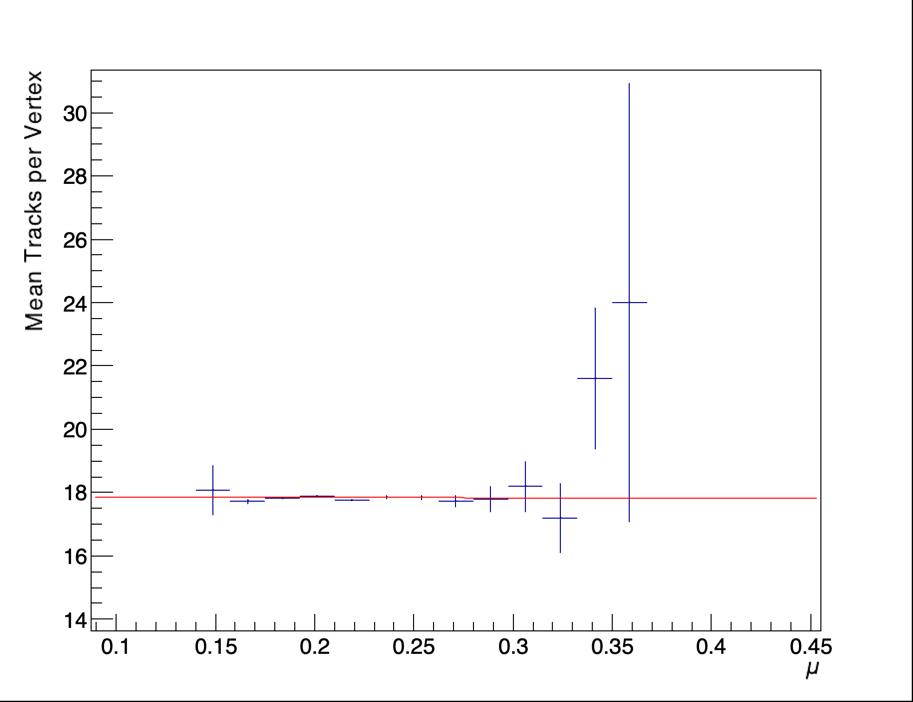
\includegraphics[width=0.32\linewidth]{images/meantpv_lowmu_mu.png}
%     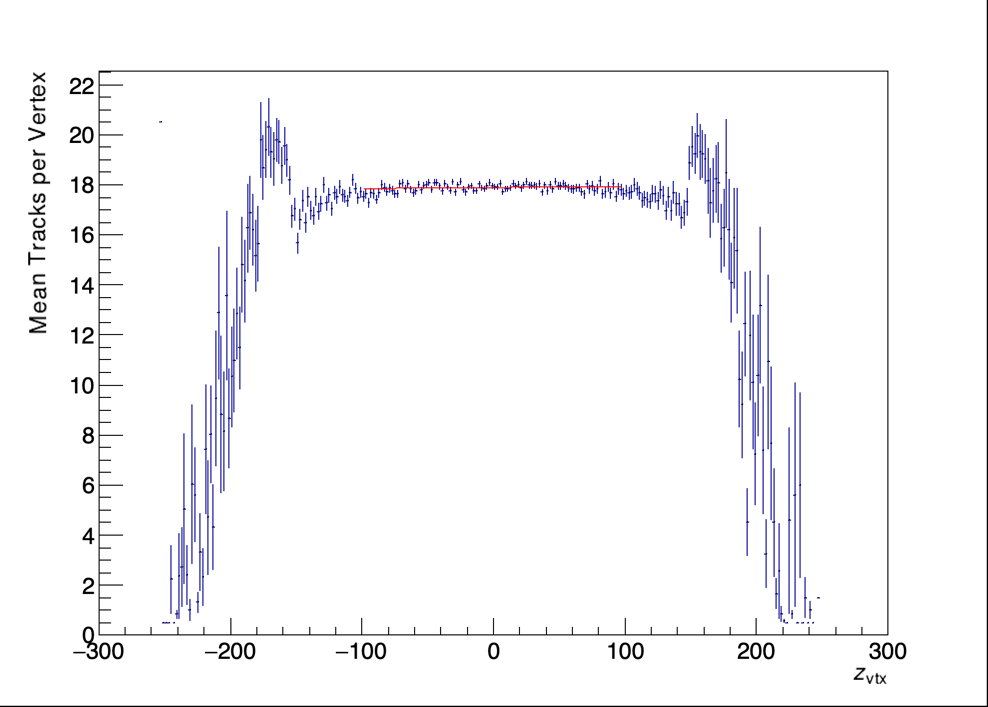
\includegraphics[width=0.32\linewidth]{images/meantpv_lowmu_zvtx.png}
%     \caption{Mean $\tpv$ in low-$\mu$ sample. Left: as a function of lumiblock number. Middle: as a function of $\mu$. Right: as a function of $z_\text{vtx}$}
%     \label{fig:lowmu_mean_tpv}
% \end{figure}